\documentclass[a4paper,fleqn]{cas-dc}
\usepackage[numbers,sort&compress]{natbib}
\usepackage{array}
\usepackage{booktabs,multirow,xcolor}
\usepackage{xurl}
\usepackage{orcidlink}
\usepackage{silence}
\WarningFilter{hyperref}{Ignoring empty anchor}
\usepackage[capitalise,nameinlink]{cleveref}
\crefname{section}{Section}{Sections}
\crefname{table}{Table}{Tables}
\crefname{figure}{Fig.}{Figs.}
\crefname{equation}{Eq.}{Eqs.}
\newcommand{\RQ}[1]{\textbf{RQ#1}}
% Latin Modern Sans for the class's sans-serif captions and tables: the T1
% default (EC sans) falls back to bitmap Type 3 fonts when cm-super is absent.
\renewcommand{\sfdefault}{lmss}
\hypersetup{hidelinks,
  pdftitle={Beyond engine latency: frequency governors and host pipelines in object detection on edge accelerators},
  pdfauthor={Dinh Thuan Nguyen; Lam Phuong Nguyen; Vinh Huy Nguyen; Sy Vu Quang; Mohan Rajesh Elara; Anh Vu Le},
  pdfsubject={Edge inference pipelines under stock DVFS governors},
  pdfkeywords={edge AI; object detection; DVFS; embedded GPU; energy efficiency; benchmarking methodology}}

\emergencystretch=3em
\hbadness=10000

\graphicspath{{figs/}}

\begin{document}

\shortauthors{D.T. Nguyen et al.}
\shorttitle{Beyond engine latency}
\title[mode=title]{Beyond engine latency: frequency governors and host
pipelines in object detection on edge accelerators}

\author[mymainaddress]{Dinh Thuan Nguyen\orcidlink{0009-0008-6467-203X}}
\ead{nguyendinhthuan.st@tdtu.edu.vn}
\author[mymainaddress]{Lam Phuong Nguyen\orcidlink{0009-0007-3439-5871}}
\ead{nguyenphuonglam.st@tdtu.edu.vn}
\author[mysecondaryaddress]{Vinh Huy Nguyen\orcidlink{0009-0006-0878-9714}}
\ead{nguyenvinhhuy@dtu.edu.vn}
\author[mythirdaddress]{Sy Vu Quang}
\ead{vuquangsy@tdtu.edu.vn}
\author[fourthaddress]{Mohan Rajesh Elara\orcidlink{0000-0001-6504-1530}}
\ead{rajeshelara@sutd.edu.sg}
\author[mythirdaddress]{Anh Vu Le\orcidlink{0000-0002-4804-7540}\corref{mycorrespondingauthor}}
\cortext[mycorrespondingauthor]{Corresponding author.}
\ead{leanhvu@tdtu.edu.vn}

\address[mymainaddress]{Faculty of Electrical and Electronics Engineering, Ton Duc Thang University, Ho Chi Minh City, Vietnam}
\address[mysecondaryaddress]{Center of Visualization and Simulation, Duy Tan University, Da Nang, Vietnam}
\address[mythirdaddress]{Advanced Intelligent Technology Research Group, Faculty of Electrical and Electronics Engineering, Ton Duc Thang University, 19 Nguyen Huu Tho Street, Tan Phong Ward, District 7, Ho Chi Minh City 700000, Vietnam}
\address[fourthaddress]{ROAR Lab, Engineering Product Development, Singapore University of Technology and Design, Singapore}

\begin{abstract}
The deployment cost of NMS-free detectors is usually
equated with the latency of the compiled engine. We measure the full
decode-to-detections pipeline of YOLO26n on a Jetson Orin Nano Super:
module input power, clocks, GPU load and official COCO accuracy
on all 5,000 val2017 images. The same FP16 TensorRT engine that takes
4.2\,ms back-to-back takes 13.2\,ms inside a sequential application,
because the stock GPU governor holds the GPU at minimum clock. A
duty-cycle model describes the measurements: engine time scales with
the inverse of the clock (validated by a fixed-frequency sweep to
4\%), interior-clock operating points sit in a 0.53--0.74
GPU-load band while floor-clock and unlocked points fall outside,
and a sequential pipeline released from the top
clock falls to the floor in seconds. Restructuring only the host
pipeline, under default governors and with identical predictions,
gives $2.4\times$ the throughput of the best sequential pipeline at
locked maximum clocks. The CPU governor is coupled to the same
loop: a sleeping CUDA wait lets \texttt{schedutil} lower the host's
clock and costs a fifth of throughput; a per-task utilization
clamp, needing no root privileges, recovers most of it at
lower energy. At camera rates below capacity, idle power sets energy
per frame and the schedule sets latency. Replications on a
Raspberry Pi~5 with Hailo-8 NPU and a Qualcomm QCM6490 (CPU and
Hexagon NPU) show the effect transfers while its mechanism shifts to
the host side. Edge-detection efficiency should be reported for the
whole pipeline under deployment governors.
\end{abstract}


\begin{highlights}
\item On Jetson, the stock GPU governor triples serial inference time.
\item Host restructuring beats a maximum-clock serial pipeline by $2.4\times$.
\item Sleeping waits down-clock the host and cost 20\% of sequential throughput.
\item At camera rates, idle power dominates energy while scheduling sets latency.
\item Pipeline gains transfer across neural accelerators, but mechanisms differ.
\end{highlights}

\begin{keywords}
Edge AI \sep Object detection \sep DVFS \sep Embedded GPU \sep
Energy efficiency \sep Jetson \sep Benchmarking methodology
\end{keywords}

\maketitle
% The template's cas-common.sty comments out \printFirstPageNotes in the
% two-column MaketitleBox, so the corresponding-author note and e-mail
% addresses are emitted manually here as an unmarked first-page footnote.
\begingroup
\renewcommand{\thefootnote}{}%
\footnotetext{\footnotesize\raggedright \textit{Corresponding author.}\\
\textit{E-mail addresses:}
\href{mailto:nguyendinhthuan.st@tdtu.edu.vn}{nguyendinhthuan.st@tdtu.edu.vn} (D.~T. Nguyen),
\href{mailto:nguyenphuonglam.st@tdtu.edu.vn}{nguyenphuonglam.st@tdtu.edu.vn} (L.~P. Nguyen),
\href{mailto:nguyenvinhhuy@dtu.edu.vn}{nguyenvinhhuy@dtu.edu.vn} (V.~H. Nguyen),
\href{mailto:vuquangsy@tdtu.edu.vn}{vuquangsy@tdtu.edu.vn} (S.~V. Quang),
\href{mailto:rajeshelara@sutd.edu.sg}{rajeshelara@sutd.edu.sg} (M.~R. Elara),
\href{mailto:leanhvu@tdtu.edu.vn}{leanhvu@tdtu.edu.vn} (A.~V. Le).}%
\endgroup

\section{Introduction}
\label{sec:intro}

Real-time object detection on embedded GPUs is usually evaluated with
two numbers per model: COCO accuracy~\cite{lin2014coco} and the latency
of the compiled engine in an isolated benchmark. Efficiency research
therefore focuses on the model: structured
pruning~\cite{li2017pruning,fang2023depgraph},
quantization-aware training~\cite{jacob2018quantization} and
distillation~\cite{hinton2015distilling} are judged by the engine
latency they remove per unit of accuracy lost. NMS-free detectors
make this framing seem even more natural. YOLOv10~\cite{wang2024yolov10}
and YOLO26~\cite{jocher2026yolo26,ultralytics2026yolo26} emit a fixed set of final detections
from a one-to-one head, so the host only decodes the image and converts
a few hundred output rows. With post-processing nearly gone, the engine
benchmark should predict the application.

\begin{figure*}[pos=t]
\centering
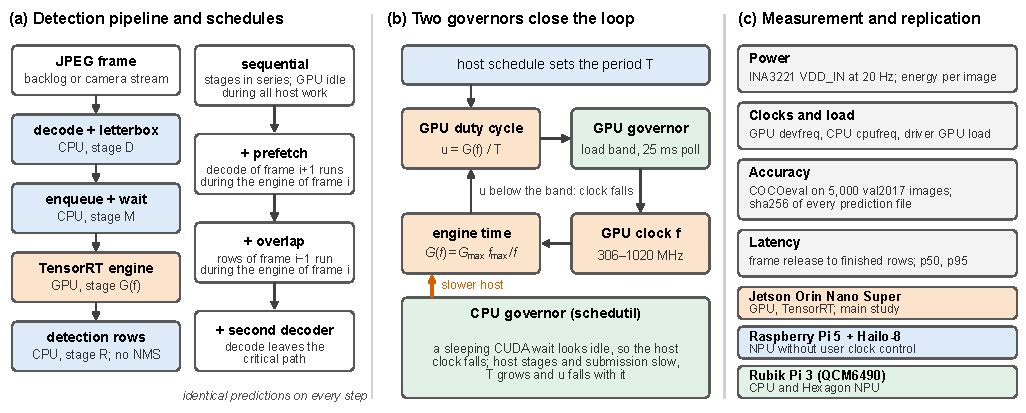
\includegraphics[width=\textwidth]{figs/framework.pdf}
\caption{Overview of the study. (a) The detection pipeline, with the
stage symbols of \cref{sec:sysmodel}, and the cumulative schedule
ladder of \cref{sec:ladder}; every scheduling step keeps the predictions
byte-identical. (b) The feedback loop described by the duty-cycle
model. The host schedule sets the period $T$ and thus the GPU duty
cycle $u$. When $u$ lies below the governor's load band, the GPU clock
falls and engine time grows. A sleeping CUDA wait also lets the CPU
governor lower the host clock, which lengthens $T$. (c) Quantities
measured on every run and the three boards of the study
(\cref{sec:setup,sec:crossplatform}).}
\label{fig:framework}
\end{figure*}

Measurements on an NVIDIA Jetson Orin Nano Super show that it does not.
Run back-to-back, the FP16 TensorRT engine of YOLO26n takes 4.2\,ms per
inference. In a conventional sequential application that decodes a
JPEG, letterboxes it, runs the engine and builds detection rows, the
same engine takes 13.2\,ms. The model, input and builder are unchanged;
the GPU's duty cycle is not. While the CPU decodes, the GPU idles, and
the stock frequency governor holds the GPU at its minimum clock of
306\,MHz, 30\% of its maximum. This also affects how compression
should be judged. A model 20\% cheaper in the benchmark would gain
little in such an application: at a fixed clock the saving is diluted
by the host stages, and the clock itself does not move.

The study did not start with governors. It first tried to make YOLO26n
cheaper through object-aware structured pruning, quantization-aware
training (QAT), distillation, compiler-guided pruning of the most
expensive head layers, and a per-image adaptive-resolution router.
These variants either lost several AP points or did not run faster once
compiled, and the router failed verification on held-out images. Only the
host pipeline was then restructured. Under the same default governors and with byte-identical
predictions, this gave $2.4\times$ the throughput of the best
sequential pipeline, even with all of that pipeline's clocks locked at
maximum. The gain over the standard Ultralytics predictor was
$6.9\times$.

This paper is a systematic measurement study of that gap, guided by
five research questions:
\begin{itemize}
\item[\RQ{1}] How does the GPU governor's response to an application's
  duty cycle determine the in-application cost of a fixed engine, and
  can a simple model describe it?
\item[\RQ{2}] Which host-pipeline decisions matter for throughput and
  energy, how large is each effect, and which of them interact with the
  governor?
\item[\RQ{3}] How do these decisions trade latency against energy when
  frames arrive at camera rates rather than as a backlog?
\item[\RQ{4}] How do model-level decisions (input resolution,
  compression, model size) rank once the pipeline is fixed?
\item[\RQ{5}] Do the findings carry over to other NMS-free detectors
  and to other accelerator architectures?
\end{itemize}

\noindent The contributions are:
\begin{enumerate}
\item A duty-cycle model of in-application engine time and energy
  (\cref{sec:sysmodel}), checked against direct measurements
  (\cref{sec:diagnosis}). Engine time scales with the inverse of the
  measured clock. The driver-reported GPU load is consistent with a
  load-band governor whose observed band is schedule-specific. A
  sequential pipeline sits at or below the top of that band even at the
  minimum clock, which is consistent with its never leaving the floor.
  Splitting energy into an idle floor and a marginal term gives an
  empirical upper envelope for the measured below-capacity streaming
  cells (\cref{sec:stream}).
\item A controlled, cumulative pipeline ablation on all 5,000 COCO
  val2017 images (\cref{sec:ladder}). Scheduling variants produce
  byte-identical predictions, so accuracy is held exactly constant.
  Each variant is reported with official COCO AP, throughput, input
  energy, GPU clock and CPU time under both default and locked clocks,
  and the number of decode workers is swept. On the sequential and
  prefetch schedules, the choice between two CUDA synchronization calls
  costs 17--20\% of throughput under the default governors. This loss
  is governor-mediated and drops below 1\% with locked clocks. On the
  full two-worker schedule the wait policy itself is free: a sleeping
  event wait matches a spinning one within 1\% under default and locked
  clocks. The 24\% that stream synchronization still costs there is a
  completion-boundary effect, identical at locked clocks. A controlled
  test traces the governor-mediated loss to the CPU governor: a
  sleeping wait lets \texttt{schedutil} lower the clock of the host's
  frequency domain. Keeping that domain busy recovers 97\% of the loss.
  A per-task utilization clamp~\cite{linux2024uclamp}, set without root
  privileges, recovers most of it at lower energy. Garbage-collection
  pauses in a typical evaluation loop also cost a fast pipeline 7.1\%
  of its measured throughput.
\item A streaming evaluation at 15, 30 and 60\,fps (\cref{sec:stream}).
  Energy per frame is set mainly by idle power. The highest-throughput
  configuration adds one frame period of latency at low rates. An
  arrival-aware variant removes this cost and keeps p95 latency at or
  below 41\,ms at all three rates.
\item An evaluation of model-level decisions under a fixed, optimized
  pipeline (\cref{sec:model}). Lower input resolution buys 27\% throughput in
  a naive pipeline but only 2--4\% in an optimized one (6--10\% with
  Python's cyclic garbage collector disabled). The compression and
  routing attempts are reported as negative results. On YOLO26s and
  YOLOv10n, the pipeline effects are comparable to YOLO26n's
  ($5.6$--$6.9\times$ over the standard predictor).
\item A replication of the core experiments on two further boards
  (\cref{sec:crossplatform}): a Raspberry Pi~5 with a Hailo-8 NPU,
  whose accelerator has no user-visible frequency control, and a Rubik
  Pi~3 (Qualcomm QCM6490), measured on both its CPU and its Hexagon
  NPU. The pipeline ladder transfers ($3.3\times$ on the Pi~5 with
  byte-identical predictions, $2.7\times$ before the wait-policy
  change). The Jetson-specific accelerator-governor signature is not
  directly observed on the NPU stacks, where the identifiable mechanisms
  shift to the host side. With CPU inference, the ladder flattens and
  sustained load becomes thermally limited. On the NPU stack, the CPU
  governor becomes the largest term (57\% on the matched overlap rungs)
  because the scheduler down-clocks the core that feeds the
  accelerator. That core falls from 2.7\,GHz (pinned) to
  0.95--1.8\,GHz, depending on how little host work the schedule leaves
  on the critical path.
\end{enumerate}

\Cref{fig:framework} gives an overview of the pipeline, the feedback
loop and the measurement setup. This paper does not propose a new
detector, compression method or governor, and pipelining itself is
standard practice. Its contribution
is the measurement and its explanation. On this class of device, the
interaction between the host pipeline and the frequency governor
determines more of the end-to-end cost than the model-level choices
that usually receive attention. All scripts, raw power traces and
prediction hashes are provided for checking and reproduction (see the
data and code availability statement).

\section{Related Work}
\label{sec:related}

\textbf{NMS-free detectors.}
Set-prediction detectors remove non-maximum suppression (NMS) by
one-to-one matching~\cite{carion2020detr}; RT-DETR made this regime
real-time on GPUs~\cite{zhao2024rtdetr}. YOLOv10 introduced consistent dual
assignments so that a convolutional YOLO can be deployed with a
one-to-one head and no NMS~\cite{wang2024yolov10}, and YOLO26 continues
this design with an end-to-end head~\cite{jocher2026yolo26,ultralytics2026yolo26}. With NMS
gone, the remaining host work is decode, letterbox, and a short
top-$k$ row conversion. This makes the rest of the pipeline more visible,
and it is why we study these models.

\textbf{Compression for edge detection.}
Structured channel pruning~\cite{li2017pruning,fang2023depgraph},
quantization-aware training~\cite{jacob2018quantization} and knowledge
distillation~\cite{hinton2015distilling} are the standard tools for
making detectors cheaper. They are usually judged by parameter count,
FLOPs or isolated engine latency. We run these tools on the same
deployment stack and report them in end-to-end units. Our
negative results do not show that compression is ineffective in
general. They show that, for a nano-scale NMS-free model on this
device, the model is not where the time goes.

\textbf{Latency prediction, DVFS and thermal control.}
nn-Meter showed that kernel-level effects make FLOPs a poor latency
proxy on edge devices~\cite{zhang2021nnmeter}. Tang et al.\ measured how
GPU core and memory frequencies change the time and energy of deep
learning workloads, and found that the effect differs across
networks~\cite{tang2019gpudvfs}. Nabavinejad et al.\ chose batch size and
GPU frequency jointly for inference under latency limits~\cite{nabavinejad2022batching}.
Other DVFS work on mobile and edge processors learns frequency policies
that avoid throttling~\cite{kim2021ztt}, models GPU latency under
DVFS~\cite{han2025dvfs}, or controls frequency per operator on
Jetson-class devices~\cite{zhang2026sparsedvfs}. SparseDVFS also
documents, as motivation, the antagonistic effect of the stock CPU and
GPU governors on a Jetson Orin Nano: the CPU governor down-clocks the
host during GPU-heavy phases, so the host is slow exactly when the GPU
next requests data~\cite{zhang2026sparsedvfs}. \Cref{sec:sched}
measures the same coupling inside a detection pipeline and traces it
to the CUDA wait policy. Work on 3D mobile games
showed that managing CPU and GPU frequencies jointly saves power compared
with independent governors, because the two processors depend on each
other's progress~\cite{pathania2014cpugpu}. Closest to our setting,
Karzhaubayeva et al.\ characterize CNN workloads on a Jetson TX2 and
design integrated CPU--GPU DVFS governors for them~\cite{karzhaubayeva2023cpugpu},
Lotus manages CPU and GPU frequencies jointly for object detectors on a
Jetson Orin Nano to stabilize latency under thermal
variation~\cite{gong2024lotus}, and Kang shows that latency estimators
for deadline-aware governors on Jetson Orin must condition on the memory
clock~\cite{kang2026emc}. All of these works set
frequencies, or batch sizes, from outside the application --- they design
or evaluate frequency-control policies. We leave the
stock governors in place and ask how an application's duty cycle
interacts with them: the schedule changes the operating state the stock
governors observe, and thereby the measured cost of an otherwise fixed
engine. We find a similar CPU--GPU governor coupling in a
detection pipeline, and we test one standard kernel mechanism, utilization
clamping~\cite{linux2024uclamp}, as a remedy that needed no root privileges on our system.

\textbf{Characterization of edge inference.}
Mittal surveyed optimized deep learning on Jetson devices, covering
precision, framework and power-mode choices~\cite{mittal2019jetson}.
Hadidi et al.\ compared frameworks and devices for edge inference and
reported that, for the same model, the choice of framework changes
inference time and energy considerably~\cite{hadidi2019edge}. These studies
measure the model, or the framework that runs it. We measure the
application around it: we hold the engine fixed and change only host
code and governor settings.

\textbf{End-to-end costs outside the model.}
The ``AI tax'' study showed that pre- and post-processing can dominate
accelerated AI applications~\cite{richins2020aitax}. On Jetson, JPEG
decode and preprocessing have been offloaded to dedicated
units~\cite{chen2026nvjpeg}, training pipelines have been characterized
for I/O pipelining and power modes~\cite{prashanthi2023jetson}, and the
latency distribution of a YOLO pipeline on Jetson Orin NX has been
modeled stage by stage as a function of image resolution~\cite{zhang2026resolution}.
MLPerf Inference standardizes measurement scenarios, separating offline
throughput from server and single-stream latency~\cite{reddi2020mlperf}.
For autonomous-driving detection, R-TOD analyzes and minimizes the
end-to-end delay from frame exposure to reported detections by
restructuring capture and pipelining (on-demand capture, zero-slack and
contention-free pipelines) without changing the
network~\cite{jang2020rtod}; our arrival-aware variant
(\cref{sec:stream}) is a simple member of the same family, and we
measure its interaction with the stock governors and the idle floor
rather than worst-case delay. We
do not claim that pipelining or preprocessing bottlenecks are new. What we
add is a measured account, on one device and stack, of how the
governor's response to the application duty cycle changes the
apparent cost of the \emph{model}. We also show how this reorders
deployment decisions such as compression and resolution.

\textbf{Adaptive resolution.}
Choosing input scale per image or frame can save compute in
detection~\cite{chin2019adascale,zhu2021drnet}. Our frozen pre-inference
router is a simple member of this family. We report it because it
failed held-out verification, and because its expected saving is smaller
than the pipeline effects we measure.

\begin{table}[t]
\centering
\caption{Positioning against the closest measurement studies. ``Freq.''
is how frequency enters the experiment: set directly by the
experimenter, replaced by a newly designed governor (``new gov.''),
or left to the stock governor and observed (``modif.'': a modified
stock governor; ``ucl.'': per-task utilization clamping). ``Pipe.'':
the whole decode-to-detections pipeline is measured, not only the
model. ``Acc.'': accuracy is held constant or verified per variant.
``Stream.'': camera-rate arrivals are measured, not only backlog
throughput. SLO: service-level objective. A dash means the work does
not address the aspect.}
\label{tab:related}
\scriptsize
\setlength{\tabcolsep}{1.6pt}
\begin{tabular}{@{}l l cccc@{}}
\toprule
Work & Workload & Freq. & Pipe. & Acc. & Stream. \\
\midrule
Tang et al.~\cite{tang2019gpudvfs} & DNN time/energy & direct & -- & -- & -- \\
Nabavinejad et al.~\cite{nabavinejad2022batching} & batching w/ SLOs & direct & -- & -- & -- \\
SparseDVFS~\cite{zhang2026sparsedvfs} & per-operator DVFS & direct & -- & yes & -- \\
Pathania et al.~\cite{pathania2014cpugpu} & 3D mobile games & modif. & partial & -- & -- \\
Karzhaubayeva~\cite{karzhaubayeva2023cpugpu} & CNNs on TX2 & new gov. & -- & -- & -- \\
Lotus~\cite{gong2024lotus} & detec., Orin Nano & new gov. & -- & -- & -- \\
Kang~\cite{kang2026emc} & gov.\ latency est. & direct & -- & -- & -- \\
AI tax~\cite{richins2020aitax} & pre/post-processing & -- & yes & -- & -- \\
Stage-wise latency~\cite{zhang2026resolution} & YOLO on Orin NX & stock & yes & -- & -- \\
This work & detection, 3 boards & stock${+}$ucl. & yes & yes & yes \\
\bottomrule
\end{tabular}
\end{table}

\Cref{tab:related} summarizes the positioning. The gap we fill is not
pipelining, preprocessing or DVFS per se, but the interaction with the
\emph{stock} governors under the application's own schedule and arrival
process, with accuracy held exactly constant so that the timing effects
are attributable.

\section{A duty-cycle model of the detection pipeline}
\label{sec:sysmodel}

A deliberately simple model organizes the measurements. Its three
parts describe how engine time depends on the GPU clock, how each
pipeline schedule sets the GPU's duty cycle, and how the governor picks
a clock for that duty cycle. A fourth relation splits energy into an
idle floor and a marginal part. \Cref{fig:framework}(b) summarizes the loop. Each part is checked
against measurements in \cref{sec:diagnosis,sec:ladder,sec:stream}.

\textbf{Pipeline stages.}
For each image, the CPU runs a decode-and-letterbox stage $D$ and,
for float-input engines only, a host normalization $N$. The GPU runs
the engine $G$, including copies, which take under 1\,ms on this
unified-memory device. A row construction stage $R$ converts the $300$
output rows to image coordinates. Let $M$ denote the remaining
per-image work of the main thread (buffer fill, enqueue, synchronization).

\textbf{Engine time.}
For a fixed engine, the GPU time at clock $f$ is modeled as
\begin{equation}
  G(f) = G_{\max}\,\frac{f_{\max}}{f},
  \label{eq:gf}
\end{equation}
where $G_{\max}$ is the time at the maximum clock $f_{\max}$. This
assumes the engine is limited by the GPU clock and not by memory. For
variable-clock runs, the time-weighted harmonic mean of the sampled
clock is used as an approximate summary consistent with \cref{eq:gf}.

\textbf{Schedules and duty cycle.}
The period $T$ between completed images, and thus throughput
$X = 1/T$, depends on which stages lie on the critical path. For
$k$ decode workers:
\begin{align}
  T_{\text{seq}} &= D + N + G(f) + R + M, \label{eq:seq}\\
  T_{\text{prefetch}} &\approx \max\!\big(\tfrac{D+N}{k},\; G(f) + R + M\big), \label{eq:pre}\\
  T_{\text{overlap}} &\approx \max\!\big(\tfrac{D+N}{k},\; R + M,\; G(f)\big). \label{eq:ovl}
\end{align}
The GPU busy fraction is $u = G(f)/T$. In the sequential schedule every
host millisecond is GPU idle time. \Cref{eq:pre} describes the prefetch
transition: host stages leave the critical path, and the
period becomes the maximum of the worker rate and the GPU-serial part.
The stage times in it are clock-dependent, so it serves as a structure
rather than a fitted predictor. \Cref{sec:diagnosis} measures them at a
down-clocked host; at the higher clocks of the prefetch rung, the
decode rate is correspondingly higher. Overlap also removes $R$
(\cref{eq:ovl}).

\textbf{Governor.}
The GPU governor (\texttt{nvhost\_podgov}) ships in NVIDIA's public
Jetson Linux kernel sources~\cite{nvidia2025jetsonkernel}. Its devfreq
sysfs node on the test device exposes only a 25\,ms polling interval
and no load thresholds. The thresholds were not derived from the
source; the governor is instead characterized empirically as a
load-band controller. The driver exposes the load it acts on through
sysfs, so the busy fraction $u$ can be checked directly
(\cref{sec:diagnosis}). The governor raises $f$ while $u$ exceeds an
upper threshold $u_{\text{hi}}$, lowers it while $u$ is below a lower
threshold $u_{\text{lo}}$, and is clamped to $[f_{\min}, f_{\max}]$. A
schedule therefore settles either at an interior clock with
$u \in [u_{\text{lo}}, u_{\text{hi}}]$ or at one of the clamps. The
measurements show a fixed point that this view implies. In
\cref{eq:seq}, $u$ increases as $f$ decreases, because a slower GPU occupies a larger share of the
period. If, even at $f_{\min}$, the sequential pipeline's busy fraction
$G(f_{\min})/T_{\text{seq}}(f_{\min})$ stays below $u_{\text{hi}}$, the
governor has no reason to raise the clock, and the application runs at
the minimum clock indefinitely, even though the GPU is busy
about half of the time (measured loads 0.46--0.66 at the floor,
\cref{sec:diagnosis}).

\textbf{Energy.}
Let $P_{\text{idle}}$ be the module input power with no workload under a
given clock policy, and $P_{\text{board}}$ the mean power during a run.
Energy per image splits as
\begin{equation}
  E = \frac{P_{\text{board}}}{X}
    = \underbrace{\frac{P_{\text{idle}}}{X}}_{\text{idle reference}}
    + \underbrace{\frac{P_{\text{board}} - P_{\text{idle}}}{X}}_{E_{\text{marg}}}.
  \label{eq:energy}
\end{equation}
The first term is an accounting reference: the idle draw of the board
in the measured power state, amortized over throughput. It is not a
universal lower bound, since a different sleep or power-gating regime
could go below it. On a backlog, a faster schedule shrinks the
idle-reference term. For a camera that delivers frames at a fixed rate
$r$ below the pipeline's capacity, the throughput is $X = r$ regardless
of schedule, so
\begin{equation}
  E(r) \approx \frac{P_{\text{idle}}}{r} + E_{\text{marg}}.
  \label{eq:stream}
\end{equation}
The schedule then affects energy only through $E_{\text{marg}}$, so
pipeline optimization should yield large energy savings on a backlog
but only small ones at fixed camera rates. \Cref{sec:stream} tests
this prediction and finds that \cref{eq:stream} with the backlog $E_{\text{marg}}$ substituted is an
empirical upper envelope for the below-capacity cells, not an exact
prediction.

\section{Experimental methodology}
\label{sec:setup}

\subsection{Platform and software}

\Cref{tab:platform} lists the platform. ``Default'' means the stock
governors: \texttt{nvhost\_podgov} for the GPU (eight
steps from 306 to 1020\,MHz) and \texttt{schedutil} for the CPU.
``Locked'' means \texttt{jetson\_clocks}, which pins the CPU, GPU and
memory controller (EMC) clocks to their
maxima~\cite{nvidia2024jetsonperf}. Readback at ${\approx}4$\,Hz, idle
and under a 15\,s inference load, confirmed the EMC pin (constant
3199\,MHz). Each locked phase
saves the default configuration to a fresh file and restores it
afterwards; governor and clock limits were read back after every phase. The two NumPy versions in \cref{tab:platform} differ
because Ultralytics 8.4.172 requires the newer release. This affects
only the short COCO row-conversion step, whose code is identical in
the custom pipelines and the baseline.

\begin{table}[t]
\centering
\caption{Platform and software. BSP is the board support package.}
\label{tab:platform}
\footnotesize
\begin{tabular}{@{}ll@{}}
\toprule
Board & Jetson Orin Nano Super Developer Kit, \\ & 8\,GB module \\
CPU & 6$\times$ Cortex-A78AE, two frequency \\
    & domains (CPUs 0--3, 4--5), 115--1728\,MHz \\
GPU & Ampere, 1024 cores, 306--1020\,MHz \\
Power mode & \texttt{MAXN\_SUPER} \\
OS / BSP & Ubuntu 22.04, Jetson Linux R36.5.2 \\
Kernel & 5.15.199-tegra \\
Cooling & fan under thermal control \\
 & (\texttt{nvfancontrol}); locked runs pin CPU, \\
 & GPU and EMC clocks, not the fan \\
CUDA / TensorRT & 12.6 / 10.3.0 \\
Detector software & Ultralytics 8.4.172 \\
Baseline runtime & PyTorch 2.5.0 (NVIDIA JetPack build) \\
Host libraries & Python 3.10.12, OpenCV 4.10.0, \\ & NumPy 1.21.5 (custom), 1.26.4 (Ultralytics) \\
Power sensor & INA3221 \texttt{VDD\_IN} (module input), \\ & 20\,Hz \\
\bottomrule
\end{tabular}
\end{table}

\subsection{Replication platforms}
\label{sec:replplatforms}

Two further boards (\cref{sec:crossplatform}) rerun
the core protocol with the smallest changes their stacks require. On
the Raspberry Pi~5, the model is the Hailo Model Zoo's precompiled
HEF (Hailo Executable Format) \texttt{yolov8n\_h8.hef}~\cite{hailo2023modelzoo} for the
Hailo-8 (INT8, NMS on chip, score threshold 0.2 fixed at compile time),
run through HailoRT~4.23.0 asynchronous pipelines with the same
prefetch/overlap/spin switches as the TensorRT pipeline. The
replication tables use short rung names: \texttt{seq} is the sequential
pipeline, \texttt{prefetch} adds decode prefetch, \texttt{full
w1}/\texttt{w2}/\texttt{w3} add post-processing overlap with one, two
or three decode workers, and \texttt{spin} replaces the sleeping wait.
Pi~5 power is the rail sum of its power-management IC (PMIC), which
covers the system-on-chip (SoC) but not the 5\,V loads (the Hailo-8
itself, the fan, USB), so Pi energies are SoC-side lower bounds.

The Rubik Pi~3 (Ubuntu 24.04.4, kernel 6.8) is measured with two
stacks. The CPU stack is ONNX Runtime~1.30.0 (default thread
settings)~\cite{onnxruntime} on the same YOLO26n ONNX graph as the
Jetson float engine. The NPU stack runs an INT8 QNN context binary of
the same graph on the Hexagon HTP, with the standard
$(1{,}84{,}8400)$ head and host NMS at the val settings. The board's
QNN~2.46 predates the QAIRT~2.49.40-built context, so the context runs
through the bundled runtime of the \texttt{qai-appbuilder}~2.50.40
wheel. This userspace is not robust under concurrent calls, so all NPU
inference is serialized on one thread and host stages overlap around
it. The board has no trustworthy power sensor; its sampler logs only
the three CPU frequency domains and the SoC thermal zone, at an
effective 13--18\,Hz rather than 20\,Hz. The Pi sampler reads the
PMIC's SoC-side rails at an effective 10\,Hz. Energy integrals are
trapezoids over the actual sample timestamps. The HTP stack is
bit-deterministic (hash-verified, as on the Jetson and Pi). The
multi-threaded CPU stack emits rows in nondeterministic order, so its
equivalence is checked on sorted prediction rows and by COCOeval on
each rung's saved predictions.

\subsection{Models and engines}

The main model is the pretrained YOLO26n
checkpoint~\cite{jocher2026yolo26} (2.57\,M parameters); generality is
tested with YOLO26s (10.0\,M) and YOLOv10n
(2.78\,M)~\cite{wang2024yolov10}. All are exported to ONNX with
\texttt{nms=False}, which yields a $(1,300,6)$ tensor of boxes, scores
and class indices with no NMS. Ultralytics 8.4.172 loads the YOLO26
head with the one-to-many branch by default, so \texttt{nms=False} was
verified to select the one-to-one (end-to-end) branch in both export
and prediction. Every engine is a
static batch-1 FP16 TensorRT engine built on the device with builder
optimization level~3~\cite{nvidia2024tensorrt}, except the
compression-screening engines of \cref{sec:model}, built at level~0
(level~3 reference rows are marked in \cref{tab:compression}). Two
engines are built from each graph:
\begin{itemize}
\item a \emph{float} engine that takes a normalized
  $1{\times}3{\times}S{\times}S$ FP32 RGB tensor, and
\item a \emph{uint8} engine whose graph begins with four ONNX operators
  (Cast, a BGR$\to$RGB Gather, Transpose, division by 255) and takes the
  letterboxed $S{\times}S{\times}3$ uint8 BGR image directly; its ONNX
  Runtime outputs are identical to the float graph's (maximum absolute
  difference 0 on test images).
\end{itemize}
The Ultralytics baseline uses an engine exported on the device by
Ultralytics from the same checkpoint (\texttt{half=True, nms=False})
with the TensorRT builder defaults (optimization level 3, as above). It
runs through \texttt{YOLO.predict} with confidence threshold 0.001 and
at most 300 detections, as the custom pipelines do.

\subsection{Pipelines}
\label{sec:pipelines}

All custom pipelines share one implementation and differ only in the
switches below, which define the cumulative ladder of
\cref{sec:ladder}. Each goes from a JPEG file to COCO-format rows:
OpenCV decode, letterbox to $S{\times}S$ with value-114 padding,
copy into a pinned host buffer, TensorRT execution, output copy, and
vectorized conversion of rows with confidence $\geq 0.001$ to
original-image coordinates.
\begin{itemize}
\item \emph{Input type}: float input with host normalization, or uint8
  input with in-graph preprocessing.
\item \emph{Synchronization}: \texttt{cudaStreamSynchronize} on the
  inference stream, or \texttt{cudaEventSynchronize} on an event
  recorded after the output copy. \Cref{sec:sched} also
  sets the CUDA device scheduling flag (\texttt{auto}, \texttt{spin} or
  \texttt{blocking-sync}) before context creation.
\item \emph{Prefetch}: one or two worker threads decode and letterbox
  upcoming images while the current image is processed.
\item \emph{Overlap}: double-buffered I/O, so rows of image $i{-}1$
  are built while image $i$ runs on the GPU. The \emph{arrival-aware}
  variant (\cref{sec:stream}) finishes the in-flight image immediately
  if the next frame is not yet available.
\item \emph{Garbage collection}: Python's cyclic collector runs by
  default; one diagnostic variant (\cref{sec:gc}) disables it for the
  timed window.
\end{itemize}

\subsection{Workloads}

\emph{Backlog}: all images are available at once and processed as fast
as possible, giving throughput and energy per image. \emph{Streaming}:
frames become available at a fixed 15, 30 or 60\,fps over the first
1,000 val2017 images. Frame latency (\cref{tab:measure}) includes any
queueing when the pipeline cannot keep up. The median (p50) and the p95 are reported; with
1,000-frame streams the p99 estimate rests on ten samples, and p95 is
the highest quantile considered stable at this size. In both workloads
the first 20 images are a warm-up and are excluded. In streaming runs
the arrival schedule is re-anchored at the end of the warm-up, so the
timed window starts with an empty queue. JPEG files are read once
before each phase, so all decodes come from the page cache.

\subsection{Measurement boundaries}

\begin{table}[t]
\centering
\caption{Measurement boundaries used throughout. The terms differ in the
host work and queueing they span and are never equated.}
\label{tab:measure}
\small
\footnotesize
\begin{tabular}{@{}ll@{}}
\toprule
Term & Span (start $\to$ end) \\
\midrule
GPU compute & device-side execution of one inference; \\
\quad (\texttt{trtexec}) & CUDA events, no host work \\
Enqueue-to-done & H2D enqueue $\to$ completion of its \\
\quad (``GPU ms'' in tables) & D2H; includes GPU queueing \\
Accelerator call & submit $\to$ completion of one NPU \\
\quad (``infer'', NPU tables) & call; incl.\ queue wait in overlaps \\
Frame latency & frame availability $\to$ finished \\
\quad (p50/p95, ``latency'') & COCO rows; backlog: decode start \\
Completion period & $1/{}$throughput over timed window \\
Energy per image & $\int P\,dt$ over window $\div$ timed images \\
\bottomrule
\end{tabular}
\end{table}

\Cref{tab:measure} fixes the boundaries of the recurring time
quantities. The model's $G$
(\cref{sec:sysmodel}) is the device-side kernel cost, measured as
\emph{GPU compute} in the engine sweep and as \emph{enqueue-to-done}
inside the pipelines. On this unified-memory board the two differ only
by the launch and copy path: 0.1--0.4\,ms at the top clock (4.25\,ms
device-side versus 4.33--4.65\,ms enqueue-to-done for the same locked
engine). At low clocks the launch path itself stretches
(\cref{sec:sched}). The $M$ term of \cref{sec:sysmodel} is host work
outside $G$ on the pipeline's critical path and never double-counts
waiting already inside an enqueue-to-done span.

\subsection{Power, clock and thermal measurement}

A separate process samples \texttt{VDD\_IN} voltage and current, the GPU
\texttt{devfreq} clock, the highest CPU core clock and the junction
temperature (\texttt{tj-thermal}) at 20\,Hz. Energy is the trapezoidal
integral of power over each run's wall-clock timed window.
\texttt{VDD\_IN} is the module's main input rail (INA3221 monitor);
carrier-board loads (fan, USB peripherals, display) sit on other rails
and are excluded. Idle power was measured twice per clock policy over
60\,s windows (\cref{sec:ladder}). Unless stated otherwise, reported GPU
clocks are arithmetic means of the samples; \cref{eq:gf} uses the
harmonic mean. To check sampler overhead, the sequential and full
pipelines were each run twice with and without the power sampler on the
first 2,000 val2017 images, with a lighter GPU load and clock logger
running in both cases. Mean throughput differed by less than 0.2\%
(40.2 versus 40.2 and 209.7 versus 209.4 images/s), well within
run-to-run variation.

\subsection{Accuracy protocol and data hygiene}

Accuracy is official \texttt{pycocotools} COCOeval (bbox, maxDets 100)
on all 5,000 COCO val2017 images~\cite{lin2014coco}, reported as AP
(IoU 0.50:0.95), AP$_{50}$ (IoU 0.50) where noted, and AP$_S$ (small
objects). Every prediction file is hashed. Pipelines that differ only
in scheduling produce byte-identical predictions in every repeat and
under both clock policies, so their accuracy is exactly constant. Every
development decision (compression screening, router fitting, router
threshold) used two disjoint 1,024-image subsets of COCO train2017: a
development split and an independent, hash-verified verification
split. The pretrained checkpoint was itself trained on train2017, so
these splits are not unseen by the base model; they are held out only
from this paper's fitting and selection, their absolute AP is
optimistic, and they serve only for relative comparisons between
variants. val2017 was used only for the measurements in this paper.

\subsection{Use of AI assistance in the measurement process}
\label{sec:aiassist}

An AI coding agent (Factory Droid) ran the campaign scripts on the
boards, transferred the traces and drafted the aggregation and
plotting code. All experiments, protocols and analysis decisions were
made by the authors, and every script was reviewed before it ran. All
tables and figures are regenerated from the archived raw traces by the
published scripts (\cref{sec:data}).

\subsection{Repetitions and statistics}

Each backlog configuration on YOLO26n is repeated three times per clock
policy. Resolution, generality, streaming and scheduling-flag
experiments are repeated twice, and locked-clock generality runs once.
Follow-up experiments from later sessions used the same software and
protocol. Driver-reported GPU load was logged in one
run per pipeline. The utilization-clamping, GIL switch-interval,
minimum-frequency CPU clamp and float-engine zero-gap \texttt{trtexec}
cells have two runs each, and the fixed-frequency sweep has three 15\,s
runs per devfreq step (\cref{sec:diagnosis}). These runs also logged
GPU load, GPU clock and the clock of CPUs 0--3 at 20\,Hz.
Configuration order is rotated between repeats, with a 10\,s pause
between runs, and no other GPU work runs during a measurement. Means and full ranges (minimum to maximum) are reported
rather than confidence intervals, because two or three repeats are too
few for a meaningful interval. Run-to-run ranges are small (median 0.8\%
of the mean for backlog throughput). The held-out router test uses a
paired image bootstrap.

\section{RQ1: The governor sets the in-application engine time}
\label{sec:diagnosis}

\subsection{Stage attribution in a sequential application}

Each stage of a conventional sequential application was first timed
with CUDA events (float-input YOLO26n engine at 640, 1,004 images of
the train2017 verification split). The medians were 7.5\,ms
for JPEG decode, 3.9\,ms for letterbox and normalization, 0.65\,ms for
the pinned host-to-device copy, 12.4\,ms for TensorRT execution and
0.01\,ms for the output copy. With row construction and Python-side
dispatch (${\approx}1.5$\,ms), the median total is 26.0\,ms for the
OpenCV-based row path (the fallback converter of the accuracy runs is
excluded). The default governors held the CPU domain near 955\,MHz, so
these are host-stage times of a down-clocked host. A clocked repeat (domain logged at 20\,Hz, 837\,MHz
mean) reproduced every stage median within 7\% (decode 8.0\,ms,
letterbox 4.2\,ms, compute 12.9\,ms, total 26.9\,ms). Copies are
negligible on this unified-memory device, and the NMS-free output needs
no suppression. By this account the model takes about half of the
application's time and is the obvious optimization target.

The same engine, however, runs in 4.1\,ms back-to-back in
\texttt{trtexec} (zero gap, two 15\,s runs, medians 4.10 and
4.13\,ms), and the uint8-input engine of \cref{tab:dvfs} in 4.2\,ms.
On val2017, every sequential pipeline of the ladder (\cref{sec:ladder})
records a mean GPU clock of exactly 306\,MHz, the governor's floor, and
a median enqueue-to-completion time of 13.2--13.3\,ms for both input
types, $3.1$--$3.2\times$ the respective back-to-back time.

\subsection{An idle-gap sweep isolates the governor}

To isolate the governor, the uint8 engines were run in \texttt{trtexec}
with a forced idle gap between inferences, twice for 15\,s per point
(\cref{fig:dvfs}, \cref{tab:dvfs}). With locked clocks, YOLO26n's
median compute time is 4.20--4.27\,ms at every gap. With default
governors it stays at 4.2--4.3\,ms up to a 2\,ms gap, then grows to
5.5\,ms at 4\,ms, 6.8\,ms at 8\,ms and 12.4\,ms at 33\,ms. YOLO26s,
which keeps the GPU busy longer per inference, holds its 6.8\,ms up to
a 4\,ms gap and rises to 20.5\,ms at 33\,ms. The gap is host idle time:
at 33\,ms the achieved rate is about 26.7 inferences/s, with no
camera-style arrival process, and because \texttt{trtexec} pipelines
its enqueues the GPU-idle interval is shorter than the requested sleep
(\cref{tab:dvfs}). Along this axis, a host that leaves
${\approx}30$\,ms between inferences pays about $3\times$ the minimum
compute time per frame under the default governor. Camera-rate arrival
is measured in \cref{sec:stream}.

\begin{figure}[pos=t]
\centering
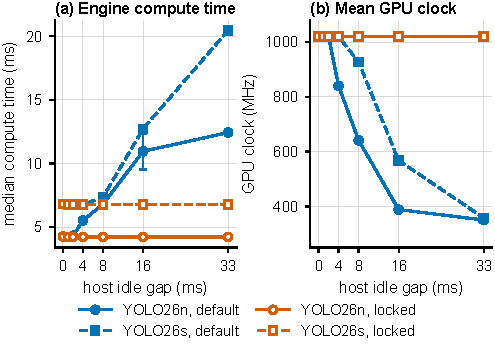
\includegraphics[width=\columnwidth]{figs/dvfs.pdf}
\caption{Median GPU compute time of the uint8 FP16 engines in
\texttt{trtexec} (left) and mean sampled GPU clock (right) versus a
forced idle gap between inferences. Mean of two 15\,s runs per point.
Default governors (blue, filled markers) versus
\texttt{jetson\_clocks} (red, open markers); circles and solid lines
show YOLO26n, squares and dashed lines YOLO26s. The
gap is host idle time (\texttt{--idleTime}), not a frame period.}
\label{fig:dvfs}
\end{figure}

\begin{table}[t]
\centering
\caption{Idle-gap sweep (\texttt{trtexec}, uint8 FP16 engines, mean of two
15\,s runs). Default governors: measured median compute time, harmonic-mean
GPU clock $\bar f$, and the prediction $G_{\max} f_{\max}/\bar f$ of
\cref{eq:gf}. ``Lock'' is the measured median with \texttt{jetson\_clocks}.
The gap axis is the requested host idle time (\texttt{--idleTime}), not a
frame period. Because \texttt{trtexec} pipelines its enqueues, the
achieved rate (last row pair) implies a mean GPU-idle interval shorter
than the requested sleep. Where the host requests 4, 8, 16 and 33\,ms,
this interval is 3.0, 5.7, 9.4 and 25.4\,ms for YOLO26n and 1.5, 4.9,
8.1 and 18.0\,ms for YOLO26s.}
\label{tab:dvfs}
\small
\setlength{\tabcolsep}{2.2pt}
\begin{tabular}{r rrrr rrrr}
\toprule
& \multicolumn{4}{c}{YOLO26n} & \multicolumn{4}{c}{YOLO26s} \\
\cmidrule(lr){2-5} \cmidrule(lr){6-9}
Gap (ms) & ms & $\bar f$ & pred. & lock & ms & $\bar f$ & pred. & lock \\
\midrule
0 & 4.25 & 1020 & 4.22 & 4.25 & 6.80 & 1020 & 6.78 & 6.80 \\
1 & 4.23 & 1020 & 4.22 & 4.22 & 6.79 & 1020 & 6.78 & 6.78 \\
2 & 4.31 & 1020 & 4.22 & 4.22 & 6.78 & 1020 & 6.78 & 6.78 \\
4 & 5.52 & 836 & 5.15 & 4.21 & 6.77 & 1020 & 6.78 & 6.78 \\
8 & 6.80 & 632 & 6.82 & 4.21 & 7.35 & 926 & 7.46 & 6.76 \\
16 & 10.95 & 355 & 12.15 & 4.21 & 12.72 & 550 & 12.57 & 6.76 \\
33 & 12.43 & 323 & 13.33 & 4.22 & 20.45 & 327 & 21.12 & 6.77 \\
\midrule
\multicolumn{9}{l}{achieved inf/s, YOLO26n: 235,\ 236,\ 169,\ 118,\ 81,\ 49,\ 27} \\
\multicolumn{9}{l}{achieved inf/s, YOLO26s: 147,\ 147,\ 147,\ 121,\ 82,\ 50,\ 27} \\
\bottomrule
\end{tabular}
\end{table}


\subsection{Validating the duty-cycle model}

\textbf{Engine time.}
\Cref{tab:dvfs} compares the measured compute time with the prediction
of \cref{eq:gf}, which uses $G_{\max}$ from the locked runs and the
harmonic-mean clock sampled during each run. Over the 14 down-clocked
sweep runs, the mean absolute error is 4.8\%, with signed per-cell
errors from $-6.7$\% (YOLO26n, 4\,ms gap) to $+11.0$\% (YOLO26n,
16\,ms gap). The largest error (23\%) occurs in one of the two
16\,ms-gap YOLO26n runs, whose median compute time differs from its
repeat's by 30\% although their harmonic-mean clocks differ by only
8\%. This suggests clock changes faster than the 20\,Hz sampling
resolves; independent measurements put the GPU clock-actuation lag
at about 5\,ms on this SoC family~\cite{kang2026emc}.

For the non-overlapped application rungs of \cref{tab:ladder},
\cref{eq:gf} overestimates the measured enqueue-to-completion time by
0.4--11.5\%. Part of this bias is expected: \cref{eq:gf} attributes all
engine time to the GPU clock, with no clock-insensitive component
(memory-bound kernels, launch overhead). The window's harmonic-mean
clock also includes host-only intervals, during which the clock is
lower. In the load-logging session, re-weighting the clock by the
driver's per-sample GPU load reduces the prefetch rungs' overestimate
from $+19$--$36$\% to $+9$--$13$\%, so much of the bias where the clock
moves is a sampling artefact of the window average. The sequential
rungs, pinned at 306\,MHz throughout, still show a $5$--$7$\%
overestimate, the cleaner estimate of the clock-insensitive share.
\Cref{eq:gf} is therefore treated as a first-order description with a
${\sim}5$\% residual, not as an exact law.

A fixed-frequency sweep avoids window averaging. With the GPU's
devfreq domain pinned at each of its eight steps (CPU and memory clocks
at their shipped settings), the uint8 engine at zero gap takes from 12.49\,ms at 306\,MHz to 4.25\,ms at
1020\,MHz (\cref{tab:fixedfreq}). A pure inverse fit $G=b/f$, with $b$
fitted by least squares, reproduces these medians with a mean absolute
error of 3.7\% but a systematic residual, positive at the floor and
negative at the top clock. The anchored form of \cref{eq:gf}
($b=G_{\max}f_{\max}$) is less accurate (6.6\% mean absolute error,
always overestimating below the top clock). The two-term fit
$G(f)=a+b/f$ removes the structure ($a=0.63$\,ms,
$b=3.63$\,GHz$\cdot$ms, mean absolute error 0.7\%, all residuals within
$\pm1.5$\%). Adding the ${\approx}0.7$\,ms launch path to the pinned
306\,MHz time reproduces the sequential pipeline's 13.2\,ms
enqueue-to-completion.

The memory (EMC) clock also scales with load on this SoC and is a
possible confound; prior work reports memory-clock effects of 11--48\%
on edge-inference latency~\cite{kang2026emc}. The sweep was therefore
rerun with three repeats per step and the EMC clock logged at
${\approx}4$\,Hz, plus two control runs with the EMC governor fully
unlocked. An attempted EMC lock did not hold; on the same SoC family,
EMC clock control is documented to fail silently on these board support
packages unless a second lock bit is asserted~\cite{kang2026emc}. The
confound is therefore controlled by measurement. The logged memory
clock is bistable across the GPU steps (\cref{tab:fixedfreq}). Fitting
$a{+}b/f$ to only the EMC-constant points changes $b$ by 2\% (3.55
versus 3.63\,GHz$\cdot$ms), and the unlocked control runs reproduce the
pinned medians within 0.4\%. The inverse trend is thus primarily a
GPU-clock effect and cannot be explained by memory-clock scaling alone.

\begin{table}[t]
\centering
\caption{Fixed-frequency sweep: the uint8 YOLO26n engine at zero idle
gap with the GPU pinned at each devfreq step (three 15\,s
\texttt{trtexec} runs per step; repeat medians agree to 1.1\%). The
memory clock is logged (constant 2133\,MHz at 306--510\,MHz,
bistable 2133--3199\,MHz from 612\,MHz up).
$G(f)=b/f$ uses the least-squares $b=3.94$\,GHz$\cdot$ms fitted to the
eight points. Anchoring $b=G_{\max}f_{\max}$ at the top point instead,
as \cref{eq:gf} does, raises the mean absolute error to 6.6\%.
The two-term fit adds
a clock-insensitive $a$. Errors are signed, (predicted $-$
measured)/measured.}
\label{tab:fixedfreq}
\small
\begin{tabular}{r rr rr}
\toprule
$f$ (MHz) & measured (ms) & $b/f$ (\%) & $a{+}b/f$ (\%) \\
\midrule
306  & 12.49 & $+3.1$ & $+0.1$ \\
408  &  9.54 & $+1.2$ & $-0.1$ \\
510  &  7.86 & $-1.7$ & $-1.3$ \\
612  &  6.48 & $-0.6$ & $+1.4$ \\
714  &  5.68 & $-2.8$ & $+0.7$ \\
816  &  5.05 & $-4.5$ & $+0.6$ \\
918  &  4.59 & $-6.5$ & $ 0.0$ \\
1020 &  4.25 & $-9.1$ & $-1.4$ \\
\bottomrule
\end{tabular}
\end{table}

\textbf{Governor operating points.}
The busy fraction $u$ of \cref{sec:sysmodel} can be estimated from
timing, but the GPU driver also reports its own load (per mille,
through sysfs). In a separate session, the eight pipeline rungs were
rerun on the first 2,000 val2017 images with this load and the GPU and
CPU clocks logged at 20\,Hz. The measured load agrees with the timing
estimate within 0.05 for every rung (the estimate is 0.01--0.05
higher) and is used for the application rungs below.

\Cref{fig:operating} plots every operating point as GPU load against
harmonic-mean clock. Whenever the governor settles clearly inside its
range (400--1000\,MHz), the load lies between 0.53 and 0.74: 0.53--0.64
for the \texttt{trtexec} sweep (timing estimate) and 0.64--0.74 for the
application rungs (measured). Two caveats apply. The two sources use
different estimators, so the lower edge cannot be separated from the
timing estimate's high bias. The 0.74 upper edge comes from a rung
settled at 993\,MHz, close to the 1020\,MHz clamp, so the true upper
threshold may lie higher. With these caveats, this is the load-band
behavior assumed in \cref{sec:sysmodel}. The sequential rungs sit at
the floor with measured loads of 0.46--0.66, at or below the observed
band's top, consistent with the governor never raising the clock (the
fixed point of \cref{sec:sysmodel}). Removing host stages from the
GPU's critical path pushes the load to the top of the band or above,
and the clock follows. Prefetch with event synchronization settles at
853\,MHz (harmonic mean) in the load-logging session and 881--891\,MHz
across the three backlog repeats; its stream-synchronized variant stays
at 655\,MHz here and at 631--694\,MHz in the blocking-sync runs of
\cref{sec:sched}. The full schedule, at a measured load of 0.87
(timing estimate 0.90), stays at 1020\,MHz.

\textbf{The floor is the only stable point observed.}
Whether a load-band controller holds a sequential pipeline at a high
clock if it starts there was tested twice: the sequential
stream-synchronized pipeline was started with locked clocks and the
default governor restored after 10\,s. At 1020\,MHz the load was only
0.35--0.36, below the band. Within 0.25\,s of the release the governor
began to step down (1020, 714, 612, 510, 408\,MHz), held 408\,MHz for
about 2.5\,s at a load of about 0.5, and reached 306\,MHz 3.3--3.4\,s
after the release, where it stayed at a load of 0.52--0.53. No run
showed a second operating point. The model does not exclude interior
equilibria (a pipeline whose load stops responding to the clock could
settle elsewhere), but for this workload the release lands at the floor
from every starting clock tested.

\begin{figure}[pos=t]
\centering
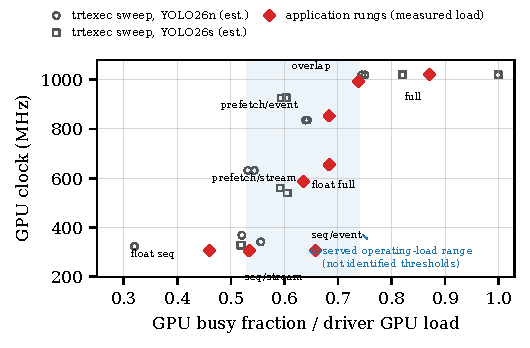
\includegraphics[width=\columnwidth]{figs/operating.pdf}
\caption{Governor operating points: GPU busy fraction or measured load versus
harmonic-mean GPU clock. Open markers: \texttt{trtexec} idle-gap
sweep, busy fraction estimated from timing. Diamonds: default-governor
application rungs (first 2,000 val2017 images), load measured by the GPU
driver. The shaded band (0.53--0.74) is the observed operating-load
range. It contains every operating point with a clock between 400
and 1000\,MHz and is not an identified pair of controller thresholds.}
\label{fig:operating}
\end{figure}

\textbf{Clock and power traces.}
In \cref{fig:traces}, both sequential variants stay at 306\,MHz,
prefetch climbs in steps from the floor and then moves between about
700 and 1020\,MHz, and the full schedule is pinned at 1020\,MHz. Input
power follows the clock. Both optimized schedules also show short power
dips whose spacing grows over the run: from about 1.9 to 4.3\,s for the
full schedule, and at longer, less regular intervals (up to about
7\,s) for prefetch. The dips were traced to Python's cyclic garbage
collector, whose pauses grow with the list of detection rows; their
effect over whole runs is quantified in \cref{sec:ladder}.

\begin{figure}[pos=t]
\centering
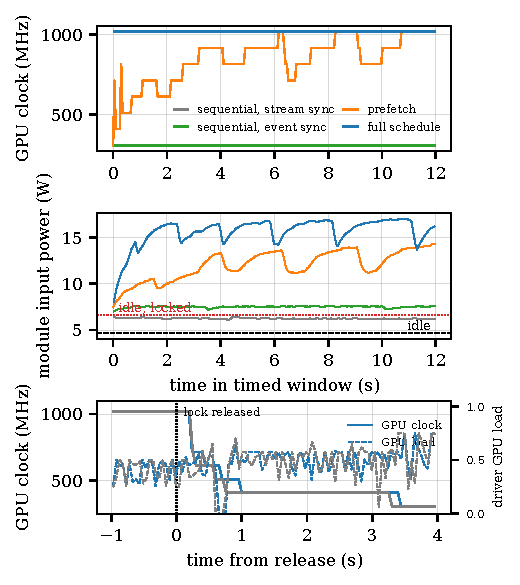
\includegraphics[width=\columnwidth]{figs/traces.pdf}
\caption{(a) GPU clock and (b) module input power during the first 12\,s
of four YOLO26n application runs on val2017 under default governors
(20\,Hz samples); the two sequential traces coincide at 306\,MHz in the
top panel. (c) The lock-then-release experiment. The sequential
pipeline is started with the GPU clock locked at 1020\,MHz, and the lock
is released at $t{=}0$ (dotted line). Clock (thick lines) and driver GPU load
(thin lines, right axis) of two repeats fall to the 306\,MHz floor within
about 3.4\,s.}
\label{fig:traces}
\end{figure}

\textbf{Answer to RQ1.}
Under the default governor, the in-application cost of a fixed engine
is set by the application's GPU duty cycle. Engine time follows the
inverse of the clock (\cref{eq:gf}). Every operating point observed
inside the governor's range sits in a GPU-load band of 0.53--0.74,
consistent with the load-band behavior of \cref{sec:sysmodel}, whose
exact thresholds are not identified. The only other observed state is
the floor. A sequential pipeline reaches it from any starting clock and
stays there, which makes its engine about $3\times$ slower than the
benchmark, a larger effect than any engine-time change produced by the
compression methods tested (\cref{sec:model}).

\section{RQ2: Which pipeline decisions matter}
\label{sec:ladder}

\subsection{Cumulative ablation on COCO val2017}

\Cref{fig:timeline} illustrates the three schedules. \Cref{tab:ladder}
and \cref{fig:ladder} report the cumulative ladder on
all 5,000 val2017 images. Model, engine and accuracy are fixed.

\begin{figure*}[t]
\centering
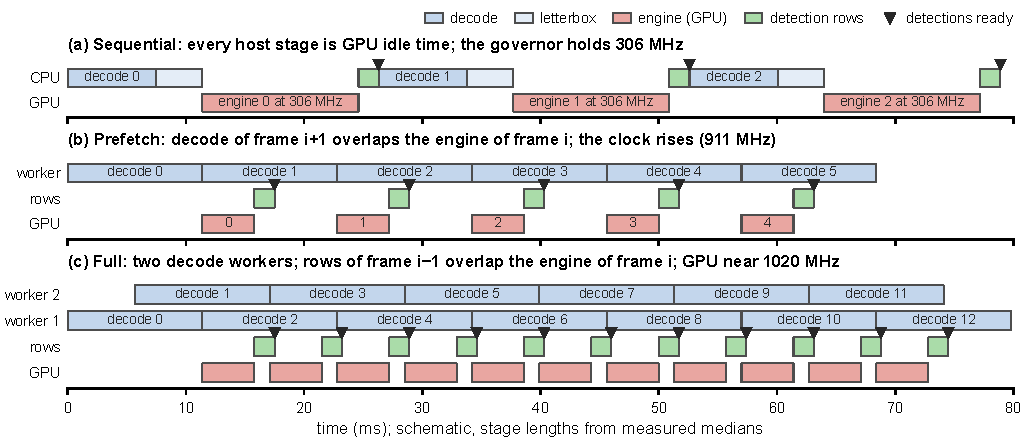
\includegraphics[width=\textwidth]{figs/timeline.pdf}
\caption{Schematic of the three schedules. The time axis uses the measured stage medians of the sequential
float pipeline of \cref{sec:diagnosis}: decode 7.5\,ms, letterbox
3.9\,ms, rows ${\approx}1.5$\,ms and engine 13.2\,ms (host-measured
enqueue-to-completion at 306\,MHz; the device-side CUDA-event share is
12.5\,ms, \cref{tab:fixedfreq}). The stage medians sum to 26.0\,ms,
while the measured period is 29.5\,ms (33.9 images/s). The difference
is per-image main-thread work outside the timed stages.
Markers ($\blacktriangledown$) show
when each frame's detections become ready. The bars show the structure,
not the measured throughputs. In (a) every host stage is GPU
idle time, so the governor holds the minimum clock. In (b) and (c) the
host stages overlap engine execution.}
\label{fig:timeline}
\end{figure*}

\begin{table*}[t]
\centering
\caption{Cumulative pipeline ablation for YOLO26n at 640 on all 5,000 COCO val2017
images (batch 1, FP16 TensorRT, \texttt{MAXN\_SUPER}). Each cell is the mean of three
rotated runs; run-to-run throughput ranges are below 2.5\% of the mean for every
cell except the float sequential pipeline under default governors (33.1--34.3 images/s) and prefetch with stream synchronization under default governors (111.5--119.1 images/s). The $\dagger$ row is a diagnostic, not a cumulative step: it reverts the previous rung's event synchronization to isolate its effect (\cref{sec:sched}). The last two rows are variants of the full uint8 pipeline.
AP is official COCOeval. Each row's predictions were byte-identical across
all six runs (both clock settings), and rows with the same input type share one
prediction file, except the Ultralytics baseline, which exports its own
engine and has its own prediction hash. GPU MHz is the mean sampled \texttt{devfreq} clock under the default
governor (always 1020 when locked). CPU ms is process CPU time per
image; W is mean module input power (\texttt{VDD\_IN} rail). Table headers
abbreviate images per second as img/s.}
\label{tab:ladder}
\small
\setlength{\tabcolsep}{3.4pt}
\begin{tabular}{lcc rrrrr rrr}
\toprule
& & & \multicolumn{5}{c}{Default governors} & \multicolumn{3}{c}{\texttt{jetson\_clocks}} \\
\cmidrule(lr){4-8} \cmidrule(lr){9-11}
Pipeline & AP & AP$_S$ & img/s & mJ/img & W & GPU MHz & CPU ms & img/s & mJ/img & W \\
\midrule
Ultralytics \texttt{predict} & 0.4026 & 0.1978 & 31.1 & 194.6 & 6.06 & 306 & 20.5 & 73.9 & 139.3 & 10.29 \\ \midrule
Ours: float input, sequential & 0.4024 & 0.1975 & 33.9 & 187.6 & 6.36 & 306 & 21.9 & 59.9 & 165.3 & 9.90 \\
+ in-graph uint8 preprocessing & 0.4026 & 0.1977 & 40.1 & 156.1 & 6.26 & 306 & 17.8 & 90.1 & 119.1 & 10.74 \\
+ event synchronization & 0.4026 & 0.1977 & 50.0 & 150.7 & 7.54 & 306 & 21.5 & 90.4 & 119.9 & 10.84 \\
$\dagger$ + decode prefetch (stream sync) & 0.4026 & 0.1977 & 116.1 & 83.7 & 9.72 & 736 & 13.5 & 158.6 & 86.2 & 13.67 \\
+ decode prefetch & 0.4026 & 0.1977 & 146.6 & 87.2 & 12.77 & 911 & 12.7 & 159.4 & 87.2 & 13.90 \\
+ post-processing overlap & 0.4026 & 0.1977 & 175.2 & 81.2 & 14.23 & 999 & 10.6 & 182.6 & 80.5 & 14.69 \\
+ second decode worker & 0.4026 & 0.1977 & 213.8 & 74.5 & 15.94 & 1019 & 11.6 & 217.9 & 74.5 & 16.24 \\ \midrule
Full scheduling, float input & 0.4024 & 0.1975 & 89.2 & 109.9 & 9.80 & 599 & 21.6 & 98.5 & 122.2 & 12.03 \\ \midrule
Full, arrival-aware overlap & 0.4026 & 0.1977 & 194.8 & 77.9 & 15.17 & 1011 & 12.8 & 214.2 & 75.2 & 16.12 \\
Full, GC paused in timed loop & 0.4026 & 0.1977 & 230.2 & 71.6 & 16.49 & 1016 & 11.2 & 231.8 & 72.4 & 16.79 \\
\bottomrule
\end{tabular}
\end{table*}


\begin{figure*}[t]
\centering
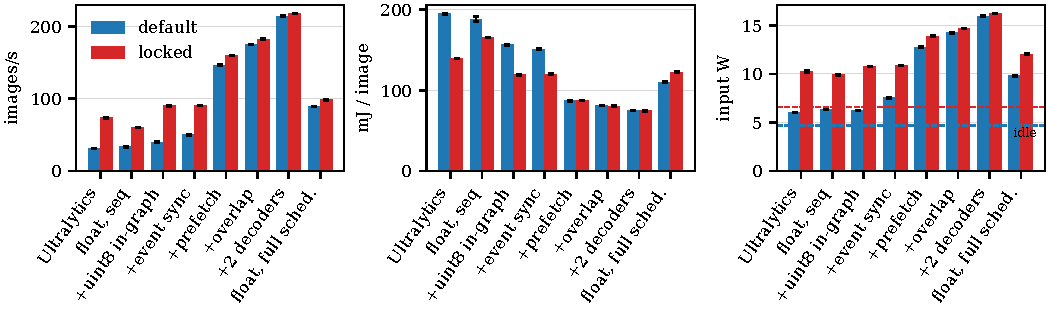
\includegraphics[width=\textwidth]{figs/ladder.pdf}
\caption{Throughput, energy per image and mean input power along the
ladder of \cref{tab:ladder} (bars: mean; whiskers: minimum--maximum of
three runs). Dotted lines in (c) mark idle input power
(4.68\,W default, 6.62\,W locked).}
\label{fig:ladder}
\end{figure*}

\textbf{Accuracy.}
The uint8 pipeline scores 0.40257 AP and 0.19766 AP$_S$, against 0.40259
and 0.19779 for the Ultralytics predictor on its own engine; the
float-input variant scores 0.40240. The ${\approx}0.6$-point gap to the
40.9 AP reported for YOLO26n on a desktop GPU with its own
export~\cite{jocher2026yolo26} is thus a property of the evaluation
stack, not of the pipeline. Agreement required one
decoder fix: an earlier version subtracted the fractional letterbox
padding instead of the integer placement offset, which shifted boxes by
half a pixel for odd padding and measurably lowered AP on the
verification split. Every pipeline was therefore checked with official
COCOeval on the full split.

\textbf{Baselines.}
Under default governors the Ultralytics predictor and the float-input
sequential pipeline reach 31.1 and 33.9 images/s, with the GPU at
306\,MHz throughout. Locking clocks with \texttt{jetson\_clocks}, the
usual benchmarking recommendation on Jetson~\cite{nvidia2024jetsonperf},
raises them to 73.9 and 59.9 images/s at 3.5--4.2\,W more input power.

\textbf{Host-side changes help a sequential schedule only through the host.}
Moving normalization and the channel transpose into the engine saves
4.1\,ms of CPU time per image and raises throughput by 18\% (33.9 to
40.1 images/s). Waiting on an event instead of the stream raises it to
50.0 images/s; equivalently, the stream-synchronized pipeline loses
20\%. The GPU clock (306\,MHz) and engine time (13.2\,ms) are
unchanged, so the gain comes from the host side, at a cost of 1.3\,W and
3.7\,ms of CPU time per image (\cref{sec:sched}).

\textbf{Overlapping CPU and GPU work changes the governor's regime.}
Prefetching the next image's decode and letterbox is the largest
single step, from 50.0 to 146.6 images/s. The GPU is now idle only
briefly, and its mean clock rises to 911\,MHz. The engine's enqueue-to-completion time falls from 13.2 to
4.4\,ms, close to its back-to-back value. Overlapping row construction
of image $i{-}1$ with inference of image $i$ gives 175.2 images/s, and a
second decode worker 213.8 images/s. More workers do not help: in a
separate sweep over one to five workers (two runs each), throughput was 174.9, 214.2, 215.9, 216.4 and
216.6 images/s, so the third to fifth workers add 1.1\% together. With
two workers the GPU's measured load is already 0.90 (0.87 in the
load-logging session of \cref{sec:diagnosis}) and
its clock is at the maximum, so the pipeline is limited by the engine
and the main thread, not by decode. Extra workers only lengthen the
queue: median per-image latency (pipeline entry to finished rows) grows
from 17.2\,ms with two workers to
30.1\,ms with five. The full pipeline is $6.9\times$ faster than the
Ultralytics predictor under default governors, but that predictor is a
weak baseline. The strongest sequential configuration
measured (uint8 input, event synchronization, all clocks locked)
reaches 90.4 images/s; the full pipeline under default governors is
still $2.4\times$ faster, at 0.4026 AP in both cases.

\textbf{Locking clocks becomes unnecessary.}
With locked clocks the full pipeline reaches 217.9 images/s, only 1.9\%
more than under the default governor, at the same 74.5\,mJ per image and
0.3\,W more power. Once the pipeline keeps the GPU busy, the stock
governor already selects the top clock. Locking speeds up the sequential
pipelines by 1.8--2.3$\times$ (2.4$\times$ for the Ultralytics
predictor).

\textbf{Preprocessing placement interacts with the schedule.}
The float-input full pipeline reaches only 89.2 images/s. Host-side normalization raises process CPU
time from 11.6 to 21.6\,ms per image, so the CPU becomes the bottleneck
(\cref{eq:ovl}) and the GPU clock averages only 599\,MHz. In-graph
preprocessing is thus worth 18\% in a sequential pipeline but
$2.4\times$ in the full one. The technique is not new (Ultralytics
8.4.172 already copies uint8 data and normalizes on the GPU); its value
depends on whether the schedule keeps the GPU busy.

\textbf{Where the energy saving comes from.}
Energy per image falls from 194.6\,mJ (Ultralytics) to 74.5\,mJ, a
factor of 2.6. By \cref{eq:energy}, most of this saving comes from
amortizing the idle floor (4.68\,W) over more images per second. The
marginal energy above idle is
44.1\,mJ per image for Ultralytics and 52.6\,mJ for the full pipeline;
across all default-governor rungs it spans 39 to 57\,mJ, against 22 to
150\,mJ for the idle-floor term. The full pipeline thus
does slightly more work above idle (higher clocks, two decoders) but
finishes much sooner. Its advantage holds on a backlog or when the
device can sleep after finishing, but not necessarily at a fixed camera
rate (\cref{sec:stream}).

\subsection{Garbage-collection pauses in the evaluation loop}
\label{sec:gc}

The power traces of the optimized schedules contain short dips
(\cref{fig:traces}). In the timed window of the full pipeline under the
default governor, each run contains six to seven dips of more than
2\,W below the median power, with onsets at about 4.1, 6.0, 8.3, 11.3,
14.8 and 19.1\,s. The intervals between dips grow from 1.9 to 4.3\,s.
This pattern matches CPython's generational garbage collector. A full
collection runs only when the number of long-lived objects has grown by
25\% since the last one, and every full collection traverses all of
them~\cite{python2024gc}. The evaluation harness, like most COCO
evaluation scripts, keeps every detection as a Python dictionary until
the end of the run. For val2017 these are 732,651 detections, each a
dictionary holding a box list, or about 1.5 million objects tracked by
the collector. Each full collection therefore stalls the main thread
for longer, the GPU drains, and the power drops.

To confirm the cause, a variant was added that performs one collection
before the timed window and then disables the cyclic collector until
the window ends. Reference counting still frees all acyclic objects, so
memory use is unaffected for this workload. The predictions are
byte-identical to the other uint8 rows (\cref{tab:ladder}). No run of
this variant contains a dip. The standard deviation of the sampled
input power falls from 0.88--0.90\,W to 0.16--0.20\,W under the default
governor and from 0.79--0.80\,W to 0.07--0.09\,W with locked clocks.
Throughput rises from 213.8 to 230.2 images/s, so the collector costs
7.1\% of the measured throughput. Energy per image falls from 74.5 to
71.6\,mJ. With locked clocks the cost is 6.0\% (217.9 versus
231.8 images/s).

This gain is not counted as a pipeline improvement. A deployed detector
would pass detections on rather than accumulate them, and its collector
would have little to scan. The effect matters for benchmarking. An
evaluation loop that accumulates results penalizes a fast pipeline more
than a slow one, because the same pauses are a larger share of a
shorter run. The pauses also arrive at irregular, growing intervals,
which inflates tail latency in long runs. All comparisons against the
Ultralytics predictor therefore use the rows with the collector
enabled, which is the more conservative choice for the proposed
pipeline. The rest of the paper follows the same rule.


\subsection{Synchronization: spinning versus sleeping}
\label{sec:sched}

To isolate the 20\% effect of the synchronization call, both calls
were crossed with the three device scheduling
flags~\cite{nvidia2024cuda} on the first 2,000 val2017 images
(\cref{tab:sched}). By default, \texttt{cudaEventSynchronize}
busy-waits, whereas \texttt{cudaStreamSynchronize} follows the device
scheduling policy, which here lets the host thread yield or sleep.

\begin{table*}[t]
\centering
\caption{Synchronization primitive $\times$ CUDA device scheduling flag (first
2,000 val2017 images, default governors, mean of two runs, uint8 engine).
``Enq.$\to$done'' is the median enqueue-to-completion wall time of one
inference (\cref{tab:measure}); CPU MHz is
the mean of the fastest core's sampled clock --- not necessarily the
core that runs the feeder thread. Run-to-run throughput spread exceeds 3\% only in the two sleeping-wait stream cells (8.6\% and 3.5\%, clock wandering between repeats); all other cells are within 3\%, and energy-per-image spread is below 1.3\% throughout.}
\label{tab:sched}
\small
\setlength{\tabcolsep}{2.4pt}
\begin{tabular}{lll rrrrrrr}
\toprule
Mode & Sync & Flag & img/s & mJ & W & GPU MHz & CPU MHz & CPU ms & Enq.$\to$done ms \\
\midrule
sequential & stream & auto & 40.5 & 157.2 & 6.37 & 306 & 1643 & 17.3 & 13.27 \\
 &  & spin & 50.0 & 151.1 & 7.55 & 306 & 1728 & 21.5 & 13.20 \\
 &  & blocking & 40.0 & 156.2 & 6.26 & 306 & 1694 & 17.8 & 13.30 \\
 & event & auto & 50.0 & 150.6 & 7.52 & 306 & 1728 & 21.4 & 13.20 \\
 &  & spin & 50.0 & 151.3 & 7.56 & 306 & 1728 & 21.4 & 13.21 \\
 &  & blocking & 49.9 & 151.0 & 7.53 & 306 & 1728 & 21.4 & 13.24 \\ \midrule
prefetch & stream & auto & 107.4 & 83.8 & 9.01 & 674 & 1647 & 14.2 & 6.25 \\
 &  & spin & 140.4 & 87.2 & 12.24 & 860 & 1727 & 13.1 & 4.63 \\
 &  & blocking & 110.6 & 84.1 & 9.31 & 694 & 1642 & 13.8 & 6.11 \\
 & event & auto & 141.5 & 86.8 & 12.28 & 866 & 1728 & 13.0 & 4.62 \\
 &  & spin & 140.5 & 86.7 & 12.18 & 862 & 1728 & 13.1 & 4.62 \\
 &  & blocking & 140.5 & 86.8 & 12.20 & 862 & 1728 & 13.1 & 4.63 \\
\bottomrule
\end{tabular}
\end{table*}


\textbf{The effect is spinning versus sleeping.}
In the sequential schedule, event synchronization gives 49.9--50.0
images/s under all three flags. Stream synchronization gives 40.5 images/s
with \texttt{auto} and 40.0 with \texttt{blocking-sync}, but 50.0 with
\texttt{spin}. The effect --- 19.8\% on the ladder rungs of \cref{tab:ladder} and 16.7\% in the pinned-CPU experiment below --- is therefore not a property of events versus streams. It depends only on whether the waiting host thread spins
or sleeps. On our software stack, \texttt{cudaEventSynchronize} spun
under every device flag, which is consistent with the CUDA documentation
tying blocking waits on an event to the \texttt{cudaEventBlockingSync}
creation flag~\cite{nvidia2024cuda}. Our events do not set it.
\texttt{auto} behaved like \texttt{blocking-sync} for stream
synchronization. Spinning costs 3.7--4.2\,ms of process CPU time per image and 1.2\,W of module input power, but because each image finishes sooner, energy per image is
4\% lower (151.1 versus 157.2\,mJ).

\textbf{Engine time is unchanged; host work slows down.}
The GPU clock is 306\,MHz and the engine's enqueue-to-completion time
is 13.2--13.3\,ms in all six sequential cells. The waking thread therefore
does not miss the completion by a measurable amount. (The span is not
pure GPU time: with the host clamped at 115\,MHz it grows to
31.5\,ms, because the enqueue-to-completion window contains the host's
launch path once the host is an order of magnitude slower than the
engine.) The difference lies
in the host stages. The per-image period grows from 20.0 to 24.7--25.0\,ms, and
the sampled clock of the fastest CPU core falls from 1728\,MHz to about
1643--1694\,MHz on average. We hypothesized that the CPU governor
(\texttt{schedutil}) causes the slowdown. It sets the clock of each
frequency domain in proportion to the scheduler's utilization estimate
of its CPUs~\cite{linux2024cpufreq}. While the host thread sleeps
through the 13\,ms engine phase, its core appears idle, and the governor
lowers the clock of the domain. The decode, letterbox and row
stages of the next image then run at the lower clock.

\textbf{A controlled test.}
To test this without changing the CPU governor, we pinned the sequential
pipeline to CPU 0 and logged the clock of its frequency domain (CPUs 0--3)
at 20\,Hz (\cref{tab:cpufreq}). With stream synchronization the domain
averaged 1069\,MHz, 62\% of its maximum, and throughput was 41.0
images/s. We then started a separate busy-loop process on CPU 1. It does
no work for the pipeline, but it keeps the shared frequency domain at
1728\,MHz. Throughput rose to 49.0 images/s, which closes 97\% of the gap
to event synchronization (49.2 images/s), and the pipeline's own CPU time
fell from 15.1 to 10.1\,ms per image. The busy loop had no effect on the
event-synchronized pipeline, which already held the clock at its
maximum. The effect is thus an interaction between the CUDA wait
policy and the CPU frequency governor, with one residual confound: a
busy loop also keeps the cluster out of deep idle states, which
shortens wake-up latency. We bounded that confound directly by
clamping the whole domain at its 115\,MHz minimum, so the governor
cannot respond no matter how busy the loop keeps the cluster: the
loop then changes nothing (7.6 versus 7.7\,images/s, under 1\%, mean
of two runs). Its $+20$\% at the shipped governor is therefore a
clock effect. This clamp test cannot rule out sub-millisecond
idle-state or wakeup effects at operating clocks --- at 115\,MHz a
fixed microsecond-scale cost is invisible next to 130\,ms frames ---
but the \texttt{uclamp} experiment below, which acts on frequency
alone and recovers about 87\% of the loss, bounds the
idle-state share to at most the remaining 13\%. A spinning wait keeps
the CPU clock high as a side effect.

\begin{table}[t]
\centering
\caption{CPU-clock test. Sequential uint8 pipeline pinned to CPU 0 (first 2,000 val2017
images, default governors, mean of two runs). ``Busy loop'' marks a separate process
spinning on CPU 1, which shares CPU 0's frequency domain; ``uclamp'' sets the pipeline's
\texttt{uclamp.min} to 1024 (bottom block, a separate session with its own stream-sync
and event-sync references). CPU MHz is the sampled clock of that domain's cluster; CPU ms counts only the pipeline
process. All runs produced identical predictions.}
\label{tab:cpufreq}
\footnotesize
\setlength{\tabcolsep}{2.0pt}
\begin{tabular*}{\columnwidth}{@{\extracolsep{\fill}}ll rrrrrrr@{}}
\toprule
Sync & Remedy & img/s & p50 & CPU & CPU & GPU & W & mJ/img \\
 & & & ms & ms & MHz & ms & & \\
\midrule
stream & -- & 41.0 & 23.8 & 15.1 & 1069 & 13.29 & 6.30 & 153.7 \\
stream & busy loop & 49.0 & 19.9 & 10.1 & 1728 & 13.24 & 7.69 & 157.1 \\
event & -- & 49.2 & 19.8 & 20.2 & 1728 & 13.21 & 7.47 & 152.0 \\
event & busy loop & 49.2 & 19.8 & 20.2 & 1728 & 13.19 & 7.96 & 161.7 \\ \midrule
stream & -- & 41.3 & 23.6 & 14.7 & 1088 & 13.29 & 6.33 & 153.2 \\
stream & uclamp & 48.0 & 20.3 & 10.5 & 1450 & 13.23 & 6.81 & 142.0 \\
event & -- & 49.0 & 19.9 & 20.2 & 1728 & 13.23 & 7.47 & 152.2 \\
\bottomrule
\end{tabular*}
\end{table}


\textbf{An unprivileged remedy.}
A busy loop on another core is a diagnostic, not a fix. Linux offers a
direct way to tell \texttt{schedutil} that a task needs a high clock:
utilization clamping~\cite{linux2024uclamp}. A task can raise its own
\texttt{uclamp.min} with \texttt{sched\_setattr}, without root
privileges on our system, and threads it creates inherit the clamp. We
set \texttt{uclamp.min} to its maximum (1024) for the stream-synchronized
pipeline, with no other change (\cref{tab:cpufreq}, bottom). The domain
clock rose from 1088 to 1450\,MHz, CPU time per image fell from 14.7 to
10.5\,ms, and throughput rose from 41.3 to 48.0 images/s. A same-session
event-synchronized reference reaches 49.0 images/s
(\cref{tab:cpufreq}), so the clamp closes about 87\% of the
sleeping-wait penalty. The recovery is partial because the clamp acts only
while the task is runnable, so the clock still decays while the thread
sleeps through the engine phase. Module input power rose by only 0.48\,W, so
energy per image fell by 7\%, from 153.2 to 142.0\,mJ. This is lower
than with the spinning wait (151.1--151.3\,mJ) or the busy loop (157\,mJ), because
the clamp raises the clock without burning a core. Per-task clamping is
therefore a practical alternative to spinning when a sleeping wait is
required, for example to free the core for other work.

\textbf{The two governors compound.}
With prefetch, sleeping waits reduce throughput from about 141 to 107--111 images/s, a 21--24\% loss. Here the GPU also suffers. The slower
host leaves the GPU idle for longer, the GPU governor settles at 674--694
instead of 860--866\,MHz, and the engine time rises from 4.6 to
6.1--6.3\,ms. A drop in the CPU clock thus lowers the GPU clock as well.
The underlying antagonism --- while the GPU computes, the host looks
idle and is down-clocked, so it runs slowly exactly when the GPU next
needs data --- has been described for the stock governors of the same
board family~\cite{zhang2026sparsedvfs}. Our measurements add to that
description in four ways: we trace the trigger to the CUDA wait policy
(spinning versus sleeping, not GPU work per se), we bound the effect
with the busy-loop and minimum-clock controls above, we test a
per-task remedy that needs no root privileges, and we observe the
effect propagating onward to the GPU clock through the duty cycle.

\textbf{The clamp also lifts the GPU clock.}
If the compounding runs from the host clock to the GPU clock, re-arming
the CPU governor should restore both. We set \texttt{uclamp.min} to
1024 on the prefetch rung, where the sleeping wait costs the most
(\cref{tab:uclamp2}, two repeats per cell, identical predictions
throughout). In the prefetch schedule with blocking synchronization
the clamp raises the feeder cores' clock (1615--1620 to
1714--1716\,MHz), the GPU's duty cycle rises with the faster
submission, and the GPU governor settles at 827--860 instead of
631--657\,MHz --- the range of the spinning and event-synchronized
variants. Engine time falls from 6.3--6.9 to 4.7\,ms and throughput
rises 34\% (101.8--104.2 to 136.3--140.2 images/s) at unchanged energy
per image (84.3 to 85.2--86.7\,mJ): the clamp recovers essentially
all of prefetch's sleeping-wait penalty, without burning a core.

\textbf{On the full pipeline the wait policy is free.}
\label{sec:waitfree}
The full two-worker schedule tells a simpler story
(\cref{tab:uclamp2}, bottom). With the decode pool active, a
\emph{sleeping} event wait --- per-frame events created with
\texttt{cudaEventBlockingSync} --- reaches 215.5--215.9 images/s,
indistinguishable from the spinning reference (215.3--215.6), with
0.3\,ms less process CPU time per image and 0.4--0.5\,mJ less energy
per image. Locking the clocks changes neither arm (215.1--215.6
sleeping, 214.7--215.5 spinning), and the clamp has nothing left to
recover (215.0--215.5). On this schedule the host never goes idle on
the critical path --- while the main thread sleeps through one
completion, two decode workers keep the domain busy --- so there is no
utilization dip for the governor to misread. The wait policy matters
only where the pipeline actually waits: the sequential rung, where
each frame sleeps through the engine phase, and prefetch, where a
single feeder does the same.

This paragraph replaces an earlier, incorrect version of the same
experiment, which we report for transparency. That version passed
\texttt{--overlap --workers 2} \emph{without} \texttt{--prefetch}; the
harness creates its decode pool only under \texttt{--prefetch}, so
those runs decoded on the main thread and their throughputs
(40.0--40.7 images/s under default governors, 86.3--89.3 locked) match
the sequential rung (40.1; 90.1 locked, \cref{tab:ladder}) within
2\%. What we had reported as a governor-independent 19\% wait penalty
of the two-worker schedule was the sequential schedule's
governor-mediated penalty, measured in disguise; a GIL switch-interval
control run on the same misconfigured cells was equally vacuous. The
harness now rejects \texttt{--workers} without \texttt{--prefetch},
and the corrected GIL control on the real two-worker schedule
(shortening the switch interval tenfold, 5 to 0.5\,ms, under locked
clocks) changes nothing either: 215.0--215.8 versus
215.1--215.6 images/s. The corrected runs also confirm the per-frame
completion boundary as the quantity that matters, next.

\textbf{Stream synchronization costs a quarter --- through its
boundary, not its wait.}
With the decode pool active, blocking \emph{stream} synchronization in
the enqueue-ahead loop still loses 24\% (163.9--165.1 versus
215.3--215.9 images/s), and it loses the same 24\% with locked clocks
(163.9--164.7), where the GPU stays pinned at 1020\,MHz. The cost is
therefore not the sleeping wait and not the governor: it is the
completion boundary. \texttt{cudaStreamSynchronize} waits for
\emph{all} work in the stream, including the frame just enqueued, so
the rows of frame $i{-}1$ are finished only after frame $i$ has
executed --- the loop degenerates to in-order completion with one
frame of slack, and the measured enqueue-to-completion window
stretches from 7.2 to 10.0\,ms. The per-frame event, spinning or
sleeping, is what preserves the overlap.

\begin{table}[t]
\centering
\caption{Wait policy and utilization clamping on the optimized
pipelines (uint8 engine, first 2,000 val2017 images, mean of two
repeats; identical predictions throughout, sha256 prefix
\texttt{df5a48fe35cd}). Prefetch rows: blocking stream
synchronization, default governors, a separate earlier session from
\cref{tab:cpufreq} with its own same-session references. Full-pipeline
rows (this session): every arm runs the decode pool
(\texttt{--prefetch --overlap --workers 2}); ``event, sleeps'' uses
per-frame events created with \texttt{cudaEventBlockingSync}; locked
is \texttt{jetson\_clocks}. \emph{CPU ms} the process CPU time per
image.}
\label{tab:uclamp2}
\footnotesize
\setlength{\tabcolsep}{2.2pt}
\begin{tabular}{@{}llll rrrr@{}}
\toprule
Pipeline & wait & clocks & clamp & img/s & CPU ms & mJ/img \\
\midrule
prefetch & stream, sleeps & default & --     & 103.0 & 14.8 & 84.3 \\
prefetch & stream, sleeps & default & uclamp & 138.3 & 10.7 & 86.0 \\
\midrule
full w2  & event, spins   & default & --     & 215.5 & 10.6 & 72.9 \\
full w2  & event, sleeps  & default & --     & 215.7 & 10.2 & 72.4 \\
full w2  & event, sleeps  & default & uclamp & 215.3 & 10.3 & 72.7 \\
full w2  & event, sleeps  & locked  & --     & 215.3 & 10.3 & 72.8 \\
full w2  & stream, sleeps & default & --     & 164.8 & 10.2 & 83.3 \\
full w2  & stream, sleeps & locked  & --     & 164.3 & 10.2 & 83.1 \\
\bottomrule
\end{tabular}
\end{table}

\textbf{Locking clocks removes the governor-mediated penalty --- where
there is one.}
\texttt{jetson\_clocks} fixes the CPU clock at its maximum as well as
the GPU clock. On the sequential and prefetch schedules, stream and
event synchronization then differ by less than
1\% (sequential: 90.1 versus 90.4 images/s; prefetch: 158.6 versus 159.4;
\cref{tab:ladder}) --- the roughly 20\% penalty on these schedules is
governor-mediated. The full two-worker schedule has no wait penalty to
remove: sleeping and spinning event waits agree within 1\% under both
governor regimes, and only the wrong synchronization boundary (stream
sync, above) costs throughput, identically at both clock settings. A
benchmark run with locked clocks would therefore see no
synchronization effect on any of these schedules except the
stream-sync boundary, while under the default governors the sleeping
wait alone costs a fifth of the sequential and prefetch schedules'
throughput.

The contrast between schedules is itself governor-dependent. The full
two-worker pipeline outperforms the event-synchronized sequential
pipeline by $4.28\times$ under the default governors (213.8 versus
50.0 images/s, \cref{tab:ladder}) but only $2.41\times$ with locked
clocks (217.9 versus 90.4). Locking the clocks does not raise the
overlapped pipeline's ceiling; it removes the sequential baseline's
self-inflicted penalty, so the reported benefit of scheduling depends
on the power-management regime of the benchmark.


\textbf{Answer to RQ2.}
The decisions that matter change the GPU's duty cycle:
prefetching ($2.9\times$), overlapping post-processing and adding a
decode worker (a further $1.5\times$), and how the host waits for the
GPU. On the sequential and prefetch schedules the wait penalty is
governor-mediated: a sleeping wait lets the CPU governor lower the
host's clock, and through it the GPU's; locked clocks nearly remove it. On the full two-worker schedule, sleeping and
spinning event waits agree within 1\% at default and locked clocks, and
only stream synchronization in the enqueue-ahead loop still costs 24\%,
identically at both (\cref{sec:sched}). In-graph
preprocessing matters once the schedule is no longer sequential.
Locking clocks only partly substitutes for a good schedule and adds
just 1.9\% to one. Finally,
garbage-collection pauses in the harness cost the full pipeline 7.1\%
of its measured throughput.

\section{RQ3: Latency and energy at camera rates}
\label{sec:stream}

A backlog is the right workload for offline processing, but a camera
delivers frames at a fixed rate. We released the first 1,000 val2017
images at 15, 30 and 60\,fps and measured, for each frame, the time from
its release to its finished detection rows, together with module input
energy per frame (\cref{tab:stream,fig:stream}). The arrival-aware variant
(\cref{sec:pipelines}) is included here. On a backlog it reaches 194.8
images/s, 8.9\% less than the full pipeline (\cref{tab:ladder}).

\begin{table*}[t]
\centering
\caption{Streaming at fixed arrival rates (first 1,000 val2017 images, YOLO26n 640,
default governors, mean of two runs). Latency runs from frame arrival to finished
detection rows (ms). Energy is module input energy per frame (mJ). ``sat.'' marks a pipeline
that cannot sustain the arrival rate. Its queue grows without bound, so the
achieved rate is given instead of latency. $^\dagger$Near-saturated
cell: the achieved rate is 29.8\,images/s against 30\,fps arrivals in
both repeats, so the queue drains too slowly to clear between bursts
and p95 includes the resulting queuing. Idle input power alone is
312, 156 and 78\,mJ per frame at 15, 30 and 60\,fps.}
\label{tab:stream}
\small
\begin{tabular}{l rrr rrr rrr}
\toprule
& \multicolumn{3}{c}{15 fps} & \multicolumn{3}{c}{30 fps} & \multicolumn{3}{c}{60 fps} \\
\cmidrule(lr){2-4} \cmidrule(lr){5-7} \cmidrule(lr){8-10}
Pipeline & p50 & p95 & mJ & p50 & p95 & mJ & p50 & p95 & mJ \\
\midrule
Ultralytics & 32.0 & 38.4 & 357 & 36.2 & 188.0$^\dagger$ & 201 & \multicolumn{2}{c}{sat.\ (31/s)} & 194 \\
Float, sequential & 39.2 & 45.2 & 361 & 32.2 & 84.3 & 204 & \multicolumn{2}{c}{sat.\ (34/s)} & 187 \\
uint8, seq., event & 27.4 & 33.4 & 353 & 21.6 & 25.8 & 203 & \multicolumn{2}{c}{sat.\ (50/s)} & 151 \\
+ prefetch & 26.8 & 33.3 & 354 & 26.7 & 33.2 & 198 & 20.9 & 99.3 & 123 \\
+ overlap, 2 workers & 85.3 & 91.8 & 352 & 51.9 & 58.7 & 196 & 35.5 & 49.1 & 117 \\
+ arrival-aware overlap & 27.0 & 33.1 & 354 & 26.5 & 33.2 & 198 & 20.7 & 40.6 & 122 \\
\bottomrule
\end{tabular}
\end{table*}


\begin{figure}[t]
\centering
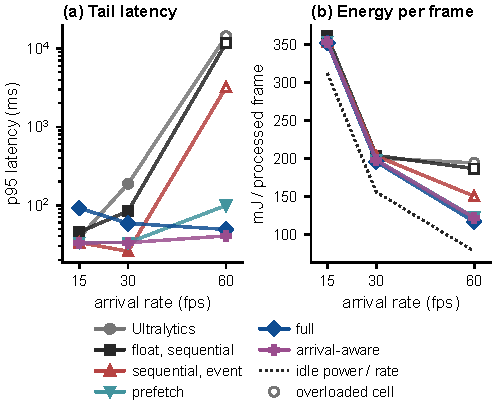
\includegraphics[width=\columnwidth]{figs/stream.pdf}
\caption{Streaming at 15, 30 and 60\,fps under default governors. Left:
p95 latency from frame release to finished rows (log scale); open
markers mark overloaded cells, where the processed rate falls short of
arrivals and the latency reflects a queue that grows over the finite
run, not a steady state.
Right: module input energy per \emph{processed} frame (the denominator
when a pipeline is overloaded); the dashed line is idle power divided by
the frame rate, the idle-reference contribution under the measured power state.}
\label{fig:stream}
\end{figure}

\textbf{Capacity.}
A pipeline that cannot sustain the arrival rate accumulates a queue,
and its latency grows with the run length. At 60\,fps this happens to
the Ultralytics predictor (31.0 images/s achieved), the float sequential
pipeline (34.2) and the uint8 sequential pipeline with event
synchronization (49.7); \cref{tab:stream} rounds these to whole images
per second. The Ultralytics predictor is also at the edge of its capacity at 30\,fps (29.8 images/s processed). Short stalls create queues that drain only slowly, and its latency distribution is strongly right-skewed (mean 55--64\,ms against medians of 36--37\,ms). An earlier harness version anchored the arrival clock before its own warm-up, which inflated exactly this tail (\cref{app:warmup}). Dropping the first 100 frames of every run moves the below-capacity p95 values by at most 4\,ms (188 to 192\,ms for the Ultralytics predictor at 30\,fps), so the remaining tails are steady-state queue drain, not start-up transients.
Capacity on a backlog therefore matters even for a camera application.
It is the margin that absorbs transient stalls.

\textbf{Energy is set by the idle floor.}
At 15\,fps every pipeline uses between 352 and 361\,mJ per frame. The
idle floor alone is 312\,mJ, or 86--89\% of the total. At 30\,fps the
spread is 196--204\,mJ against a floor of 156\,mJ. The full pipeline,
which uses 2.6$\times$ less energy per image than the Ultralytics
predictor on a backlog, uses only 2.5\% less at 30\,fps (195.7 versus
200.7\,mJ). Only at 60\,fps, where the slow pipelines saturate, does
the schedule decide energy again: 117--123\,mJ for the pipelines that
keep up, against 151--194\,mJ for those that do not, measured per
processed frame. This is the behavior described by \cref{eq:stream}. Using the idle power and the marginal energy measured on the backlog, \cref{eq:stream} with the arrival rate substituted agrees with every below-capacity streaming cell within $-0.2$ to $+11.6$\% (mean $+4.6$\%); the one slightly negative cell (Ultralytics at 15\,fps) lies inside the repeat spread of the backlog marginal estimate. For the three pipelines that saturate at 60\,fps the arrival-rate substitution underestimates by 10--37\%, because a queued pipeline never returns to the idle state the model assumes; substituting each pipeline's measured processed-frame rate instead (as the published aggregates do) brings the error on those cells to 0.3--0.5\%. The agreement below capacity comes mostly from the idle term, which dominates at camera rates. The marginal term alone is overestimated by 21--39\% for the uint8 pipelines running below capacity; for the two float-input pipelines it agrees within $-1.9$ to $+3.3$\%. The clock gap between the backlog and the stream does not explain the uint8 gap: the worst cell (the event-synchronized sequential pipeline at 15\,fps, $+39$\%) runs at 306\,MHz on both. The likely residue is CPU-side --- sleep and wake energy around each frame that the backlog marginal never pays. Whatever its origin, the backlog marginal energy is an empirical upper
envelope for the streaming marginal energy in every uint8 configuration we
measured, and is within 2--3\% of it for the float-input ones, not a prediction of it. At 15 and 30\,fps the GPU runs at about 306\,MHz in all
pipelines, so the marginal energy per frame is lower than on the
backlog, where the optimized pipelines run at about 1\,GHz. In this
regime the governor does what it is designed to do.

A corollary concerns clock locking. With \texttt{jetson\_clocks}, the
idle floor rises from 4.68 to 6.62\,W. At 30\,fps that is 221\,mJ per
frame before any work is done, already 8--13\% more than the total energy
of every default-governor pipeline in \cref{tab:stream}. For a camera
application below its capacity, locking clocks is an energy cost
without a throughput benefit.

\textbf{Latency is set by the schedule.}
At low rates the overlapped schedule has the worst latency of all
pipelines, despite having the highest backlog throughput. Its median
latency at 15\,fps is 85.3\,ms, against 27.4\,ms for the sequential
pipeline and 26.8\,ms for prefetch. Overlap finishes the rows of frame $i$ only
after frame $i{+}1$ has been decoded and enqueued, so every result
waits about one inter-arrival period (66.7\,ms at 15\,fps). The penalty
shrinks as the rate grows (51.9\,ms at 30\,fps, 35.5\,ms at 60\,fps).
The sequential pipeline is the fastest per frame at 30\,fps (median 21.6,
p95 25.8\,ms), and it keeps up with margin to spare (its backlog
capacity of ${\approx}50$\,images/s exceeds the 30\,fps arrival rate by
two thirds), but at 60\,fps it fails.
Plain prefetch keeps up at 60\,fps, but its p95 rises to 99.3\,ms. At
60\,fps the governor runs prefetch at about 410\,MHz, so its margin
over the arrival rate is small and transient stalls build queues.

The arrival-aware variant combines the two behaviors. When the next
frame is not yet available, it finishes the in-flight frame instead of
holding it. When frames queue up, it overlaps as before. Its p95 latency is within 7.4\,ms of the best pipeline at every rate (p95 33.1, 33.2 and 40.6\,ms at
15, 30 and 60\,fps), it is the only pipeline whose p95 stays at or below
41\,ms at all three rates, and its energy is within 0.4--4.3\% of the
full pipeline. Its predictions are byte-identical to the other uint8
pipelines.

The latency of the sequential pipeline also depends on the CPU
governor. Its median falls from 27.4\,ms at 15\,fps to 21.6\,ms at
30\,fps, although the work per frame is the same. At the lower rate the
CPU is idle for longer between frames, and its CPU time per frame rises
from 23.5\,ms at 30\,fps to 29.4\,ms at 15\,fps. This is
consistent with \cref{sec:sched}'s backlog finding ---
\texttt{schedutil} lowers the clock while the waiting thread sleeps
--- but we did not log the CPU clock in the streaming runs, so we
offer it as a plausible mechanism rather than a demonstrated one.

\textbf{Answer to RQ3.}
At camera rates below a pipeline's capacity, energy per frame is
dominated by the idle floor. The pipelines we tested differ by at most 2.5\% at 15\,fps and 4.2\% at 30\,fps. The schedule mainly determines
latency and capacity margin. The schedule with the best backlog
throughput has the worst latency at 15\,fps, because it holds every
result for one frame period. An arrival-aware schedule removes this
penalty at a cost of 8.9\% of backlog throughput and at most 4.3\% of
energy. Locking clocks raises the idle floor and is counterproductive
in this regime.

\section{RQ4: Model-level decisions under a fixed pipeline}
\label{sec:model}

\subsection{Compression screening and a resolution router: negative results}
\label{sec:compression}

Before the pipeline study, we spent most of our effort on the model:
L1 and gradient-based channel pruning, mixed-precision QAT,
distillation, and a per-image router that chooses between a 512 and a
640 engine from pre-inference statistics. Under a common short
recovery budget (1,024 development images, five epochs, one seed) none
of the compressed variants reduced compiled engine time at acceptable
accuracy, and the router, which looked favorable on its fitting split,
lost AP and small-object recall on an independent hash-verified
verification split, so we rejected it. \Cref{app:compression} reports
both campaigns in full. These results do not show that compression
cannot work. They show something narrower: for a 2.6\,M-parameter
NMS-free detector on this device and budget, the achievable
engine-time savings are a small fraction of the 3$\times$ governor
effect of \cref{sec:diagnosis} --- which is why the rest of this
section varies resolution and model size while holding the
optimization budget fixed.

\subsection{The value of a lower input resolution depends on the schedule}
\label{sec:resolution}

Lowering the input resolution is the cheapest model-level saving
available. It needs no training, only a new engine. \Cref{fig:resolution}
compares static 512, 576 and 640 engines of the same pretrained YOLO26n
checkpoint on all of val2017, in the naive pipeline (float input,
sequential, stream sync) and in the full pipeline. Accuracy falls from
0.4026 AP (640) to 0.3864 (576) and 0.3748 (512). AP$_S$ falls from 0.198
to 0.175 and 0.160. In the naive pipeline, 512 buys 27\% more throughput
(34.3 to 43.4 images/s) and 22\% less energy per image. In the full
pipeline the same saving shrinks to a few percent: 214.6, 222.2 and
218.7 images/s for 640, 576 and 512 ($+3.5$\% and $+1.9$\%; the
repeat ranges of the lower resolutions lie above the 640 range, so
the gain is small but consistent across the two repeats). The pipeline is now limited by the main thread
(\cref{sec:ladder}): at 1020\,MHz the engine's 4.2\,ms sits just below
the ${\approx}4.7$\,ms per-image period the host stages impose, so most
of the engine time saved by a smaller input is absorbed by the
unchanged per-image host work.

Part of that saturation is Python. Re-running the same comparison with
CPython's cyclic garbage collector disabled (\texttt{gc.disable()},
identical predictions) raises all three throughputs to 229.9, 244.0 and
252.1 images/s, and the resolution spread widens to $+6.1$\% (576) and
$+9.7$\% (512). Cyclic-GC pauses on the main thread absorb a further
share of the saved engine time; with them removed, a lower input
resolution still buys roughly a third of what it buys in the naive
pipeline, not a negligible amount. The host work that remains ---
the main thread's per-image period
(\cref{sec:ladder}) --- depends on the source image and the pipeline,
not on the network input. The energy benefit is robust either way:
73.7 to 58.0\,mJ per image (21\%) on a backlog with the default
collector, and 71.2 to 55.8\,mJ (22\%) with it disabled, because the
GPU finishes each inference sooner. The same 2.8 AP
points therefore buy a large throughput gain in a naive pipeline and a
much smaller one in an optimized pipeline --- $2$--$10$\% depending on
host-runtime hygiene. A compression or resolution decision evaluated in a naive
pipeline, or in \texttt{trtexec}, does not carry over to an optimized one.

\begin{figure}[t]
\centering
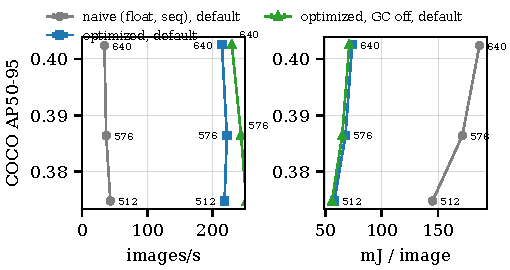
\includegraphics[width=\columnwidth]{figs/resolution.pdf}
\caption{COCO val2017 AP against throughput (images/s) and energy per
image (mJ) for
static 512/576/640 YOLO26n engines, default governors, mean of two runs
(whiskers: repeat min/max; labels: input size).
In the full pipeline (squares), lower resolution buys only $2$--$4$\%
throughput because the pipeline is limited by the main thread, not by
GPU throughput (the GPU already runs at its maximum clock); disabling
CPython's cyclic GC (triangles, identical predictions) raises all three
points and widens the spread to $6$--$10$\%.}
\label{fig:resolution}
\end{figure}


\subsection{Generality: YOLO26s and YOLOv10n}
\label{sec:generality}

\begin{table*}[t]
\centering
\caption{Other NMS-free detectors on all 5,000 val2017 images, 640, batch 1
(default: mean of two runs; locked: one run). ``Naive'' is float input with sequential execution and
stream synchronization; ``full'' is uint8 input, two prefetch workers, overlap
and event synchronization. MHz is the mean sampled GPU clock under the
default governor.}
\label{tab:generality}
\small
\setlength{\tabcolsep}{2.6pt}
\begin{tabular}{llcc rrrr rr}
\toprule
& & & & \multicolumn{4}{c}{Default} & \multicolumn{2}{c}{Locked} \\
\cmidrule(lr){5-8} \cmidrule(lr){9-10}
Model & Pipeline & AP & AP$_S$ & img/s & mJ & W & MHz & img/s & mJ \\
\midrule
YOLO26s & Ultralytics & 0.4769 & 0.3020 & 25.1 & 263.5 & 6.62 & 306 & 63.0 & 194.4 \\
 & Ours, naive & 0.4770 & 0.3019 & 24.5 & 271.6 & 6.66 & 306 & 52.2 & 221.8 \\
 & Ours, full & 0.4769 & 0.3019 & 140.1 & 131.8 & 18.47 & 1019 & 140.4 & 133.3 \\ \midrule
YOLOv10n & Ultralytics & 0.3836 & 0.1901 & 30.8 & 198.4 & 6.12 & 306 & 73.0 & 144.5 \\
 & Ours, naive & 0.3837 & 0.1900 & 33.5 & 189.4 & 6.34 & 306 & 60.0 & 167.4 \\
 & Ours, full & 0.3839 & 0.1901 & 212.4 & 76.9 & 16.33 & 1018 & 215.2 & 77.8 \\
\bottomrule
\end{tabular}
\end{table*}


\Cref{tab:generality} repeats the three main configurations for
YOLO26s (10.0\,M parameters) and YOLOv10n. In every case the three
pipelines agree in AP to within $4\times10^{-4}$, and the naive
pipelines run the GPU at 306\,MHz under default governors. YOLOv10n
behaves like YOLO26n: 30.8 images/s with Ultralytics and 212.4 with the
full pipeline ($6.9\times$), at 76.9 instead of 198.4\,mJ per image.
YOLO26s has $3.9\times$ the parameters of YOLO26n and a $1.6\times$
longer engine time (6.78 versus 4.22\,ms back-to-back). Its full
pipeline is limited by the GPU rather than the CPU. It reaches
140.1 images/s ($5.6\times$ Ultralytics), 95\% of the 146.9
inferences/s that \texttt{trtexec} achieves back-to-back, and locking
clocks does not change it (140.4). Under the default governors, the full
YOLO26s pipeline outruns the Ultralytics YOLO26n predictor with locked
clocks (140.1 vs.\ 73.9 images/s) at 0.074 higher AP and 7.5\,mJ less
per image (131.8 vs.\ 139.3). This comparison changes the pipeline and
the model at once, so it does not show that the larger model is the
better choice; YOLO26n in the same full pipeline is faster still. It
shows that the larger model costs less than a naive pipeline, even one
running with locked clocks. A deployment decision that compares model
sizes in a naive pipeline therefore mostly measures the pipeline.


\textbf{Answer to RQ4.}
Once the pipeline is fixed, model-level savings matter much less than
the engine benchmark suggests. A 2.8-point AP sacrifice for a lower
resolution yields 27\% more throughput in a naive pipeline but only
2--4\% in an optimized one (6--10\% with cyclic GC disabled), plus lower
energy on a backlog. Our
compression variants did not reduce compiled engine time at
acceptable accuracy within the budget screened.
The router saved at most one eleventh of what scheduling saved, and it failed held-out verification. Whether the schedule effects carry over to other detectors and other accelerators is \RQ{5} (\cref{sec:crossplatform}); within this section, YOLOv10n and YOLO26s show speedups of $5.6$--$6.9\times$ over the Ultralytics predictor, and for YOLO26s, whose engine is $1.6\times$ slower than YOLO26n's, the pipeline effect is large enough that the choice of pipeline matters more for throughput than the choice between the two model sizes.


\section{RQ5: Cross-platform replication}
\label{sec:crossplatform}

The Jetson study above traces the in-app cost to one mechanism: an
accelerator governor that reacts to the duty cycle the host pipeline
creates, coupled to a CPU governor that reacts to how the host waits.
How much of this is specific to that one board? We repeated the core
experiments on two boards with different accelerator architectures
(\cref{tab:boards}): a Raspberry Pi~5 whose Hailo-8 is a fixed-function
INT8 NPU with on-chip NMS and no user-visible frequency control, and a
Rubik Pi~3 (Qualcomm QCM6490), which we measure twice: on its CPU under
a three-cluster \texttt{schedutil} DVFS, and on its Hexagon HTP NPU
through a separately obtained QNN runtime. On both boards we kept the
protocol of
\cref{sec:setup}: official COCOeval on val2017 (all 5,000 images for
accuracy; the ladder uses the first 1,000 on the slower Rubik), the
same letterbox geometry and row conversion, hashed predictions, a
rotated two-repeat campaign, and clock, thermal and (where available)
power logging at 20\,Hz on the Jetson; the Pi's PMIC sustains 10\,Hz
and the Rubik sampler 13--18\,Hz (clocks and thermals only, no power,
\cref{sec:setup}). Two phases deviate from that template, and
we flag them where they appear: the pinned-frequency probes are
single runs per frequency, and the HTP streaming phase assigns the
two rotated repeats one per governor, so each HTP streaming cell is
a single run.

\begin{table*}[t]
\centering
\caption{Replication platforms. The Rubik Pi~3 is measured with two
inference stacks: its CPU, and its Hexagon NPU.}
\label{tab:boards}
\small
\begin{tabular}{@{}llll@{}}
\toprule
 & Raspberry Pi 5 + Hailo-8 & Rubik Pi 3 (CPU) & Rubik Pi 3 (NPU) \\
\midrule
SoC & BCM2712 & QCM6490 & QCM6490 \\
CPU & 4$\times$ A76, one domain, & 8 cores, three domains, & (same) \\
    & 1.5--2.4\,GHz & 0.8--2.7\,GHz & \\
Accelerator & Hailo-8 NPU (INT8), & none used & Hexagon HTP V68 \\
 & on-chip NMS & & (INT8) \\
Model & YOLOv8n HEF & YOLO26n ONNX & YOLO26n QNN ctx, \\
 & & $(1{,}300{,}6)$ & $(1{,}84{,}8400)$, host NMS \\
Runtime & HailoRT 4.23.0 & ONNX Runtime 1.30.0 & qai-appbuilder 2.50.40$^{b}$ \\
CPU governor & \texttt{ondemand}, \texttt{performance} & \multicolumn{2}{l}{\texttt{schedutil}, \texttt{performance}} \\
Power sensor & PMIC rails, SoC side only$^{a}$ & \multicolumn{2}{l}{none usable$^{c}$} \\
\bottomrule
\multicolumn{4}{@{}l@{}}{\scriptsize $^{a}$Excludes the 5\,V loads: the Hailo-8, fan and USB.}\\
\multicolumn{4}{@{}l@{}}{\scriptsize $^{b}$PyPI wheel bundling libQnnHtp + V68 skel; the board's QNN 2.46 predates the}\\
\multicolumn{4}{@{}l@{}}{\scriptsize QAIRT 2.49.40-built context binary.}\\
\multicolumn{4}{@{}l@{}}{\scriptsize $^{c}$The board's battery manager reports inconsistent values; we log clocks and thermals only.}
\end{tabular}
\end{table*}

\subsection{Raspberry Pi 5 with a Hailo-8 accelerator}
\label{sec:pi}

The Hailo model-zoo YOLOv8n HEF offloads the whole network, including
NMS, to the NPU; the host decodes, letterboxes into a uint8 NHWC buffer
and converts the NMS output to COCO rows. The vendor benchmark
(\texttt{hailortcli benchmark}) reports 431.6 images/s in throughput mode,
under both CPU governors; the NPU clock is not user-controllable, and
no register exposes it, so we cannot observe it directly. The per-call
NPU time we can measure includes host-side waiting inside the runtime;
once that share is accounted for, the residual gives no sign of a
duty-cycle response (below). A conventional sequential application on the same HEF
reaches 65.7\,images/s, 15\% of the benchmark. The in-app gap exists on
this accelerator too; with no observable accelerator clock we cannot
rule in or out an internal NPU DVFS, but the mechanism we can identify
is host-side, and the per-call NPU time, once its host-side wait share
is accounted for (below), gives no sign of a duty-cycle response.

\Cref{tab:piladder} shows the pipeline ladder. The mechanisms transfer.
Prefetching decode nearly doubles throughput ($1.86\times$), overlapping
post-processing and adding a second decode worker gives another
$1.5\times$, and a third worker adds nothing, the same saturation point
as on the Jetson. In total the restructuring reaches $2.7\times$ the
sequential application ($3.3\times$ with the spinning wait, see
below), with byte-identical predictions in every rung,
repeat and governor (sha256 prefix \texttt{455ea22b07f1}; official AP
0.320, AP$_S$ 0.122 on all 5,000 images). The wait-policy effect also
appears here, but with a different mechanism than on the Jetson:
replacing the sleeping wait on the asynchronous
inference handle with a spinning wait gains 22\% under
\texttt{ondemand} (177.9 to 217.5\,images/s) and 29\% under
\texttt{performance} (169.9 to 219.8\,images/s), where the CPU clock
is pinned at 2.4\,GHz. The gain therefore cannot be mediated by the
CPU governor; it sits inside HailoRT's wait and callback path, which
we did not profile further. A separate governor effect exists but is
smaller: a controlled probe (\texttt{seq} versus \texttt{seq} with a
busy spinner) shows the governor holding 2.4\,GHz instead of
2.2\,GHz, worth 7.7\% of throughput at 42\% more energy. The NPU time itself, measured from
submission to completion, stays at 6.3--9.3\,ms across the whole ladder
and does not respond to duty cycle; the wait time inside that interval
absorbs the schedule differences. Energy per image falls 1.8$\times$
from sequential to the best variant. We stress that these milliJoules
cover only the SoC rails; the NPU's own draw is on the unmonitored
5\,V input. These values therefore compare SoC-side energy only: they
do not establish whole-system energy rankings, because the unmeasured
Hailo-8 energy can itself move with the schedule. Within-platform
SoC-side comparisons remain meaningful between configurations that share the
same engine and accuracy; cross-engine energy comparisons on this
board need module-level power measurement. Streaming at 15, 30 and
60\,fps is consistent with the Jetson's idle-floor pattern:
sequential and overlapped pipelines differ by 9\% in energy per frame
at 15\,fps (102.0 versus 111.1\,mJ, SoC side) and converge at
60\,fps (37.4 versus 36.2\,mJ). Two cautions apply: the two-repeat
spread on the 15\,fps overlapped cell reaches 19\% (101--121\,mJ),
so that gap is indicative rather than established, and the sequential
pipeline already sits at the idle floor within measurement error (the
idle reading is a single 60\,s window: $1.534$\,W $\Rightarrow$
102.3\,mJ per frame at 15\,fps).

\begin{table}[t]
\centering
\caption{Pipeline ladder on the Pi 5 + Hailo-8 (5,000 val2017 images,
mean of two rotated repeats; p50 is the median per-image end-to-end
pipeline latency; power is SoC-side only).}
\label{tab:piladder}
\footnotesize
\setlength{\tabcolsep}{3.4pt}
\begin{tabular}{@{}llrrrr@{}}
\toprule
Governor & Rung & img/s & p50 ms & SoC mJ/img & CPU MHz \\
\midrule
\multirow{6}{*}{\texttt{ondemand}}
 & seq           &  65.7 & 15.1 & 34.2 & 2020 \\
 & prefetch      & 122.0 & 16.1 & 25.5 & 2243 \\
 & full w1       & 149.8 & 14.6 & 23.0 & 2377 \\
 & full w2       & 177.9 & 25.2 & 25.2 & 2319 \\
 & full w2 spin  & 217.5 & 21.4 & 19.4 & 2300 \\
 & full w3       & 174.7 & 31.5 & 25.2 & 2327 \\
\midrule
\multirow{6}{*}{\texttt{performance}}
 & seq           &  74.6 & 13.3 & 34.8 & 2400 \\
 & prefetch      & 120.5 & 15.1 & 26.1 & 2400 \\
 & full w1       & 140.7 & 14.7 & 22.8 & 2400 \\
 & full w2       & 169.9 & 25.5 & 26.3 & 2400 \\
 & full w2 spin  & 219.8 & 21.2 & 20.0 & 2400 \\
 & full w3       & 166.4 & 32.1 & 27.2 & 2400 \\
\bottomrule
\end{tabular}
\end{table}

Two differences from the Jetson matter. First, accuracy is not
comparable across the boards: the HEF's on-chip NMS is compiled with a
score threshold of 0.2, which truncates the low-score tail that COCO AP
rewards; AP comes out at 0.320, against the 0.373 that Ultralytics
reports for the same network at the conventional 0.001
threshold~\cite{ultralytics2023yolov8}. The threshold explains the
direction and plausibly most of the magnitude, but without pre-threshold
rows we cannot rule out smaller contributions from the HEF toolchain
itself. Because every rung produces
byte-identical predictions, this cancels in all within-platform
comparisons. Second, the default \texttt{ondemand} governor costs less
here than \texttt{nvhost\_podgov} costs on the Jetson: it sits at
2.0\,GHz even in the sequential pipeline and closes most of the gap to
\texttt{performance} once the pipeline is overlapped (219.8 versus
217.5\,images/s for the best rung). The Jetson's threefold governor effect
is specific to its aggressive GPU governor; what generalizes is that
the benchmark number describes a duty cycle the application creates,
not a property of the accelerator. One anomaly we cannot explain from
clocks alone: on the overlap rungs the shipped \texttt{ondemand}
governor is 5--6\% faster than the pinned \texttt{performance}
governor (177.9 versus 169.9\,images/s at \texttt{full\_w2}), while
with the spinning wait the order inverts (217.5 versus 219.8).
NPU-side power states may differ between the two settings; we did not
pursue it.

\subsection{Rubik Pi 3: inference on the CPU}
\label{sec:rubik}

The Rubik Pi~3 runs the same YOLO26n ONNX graph as the Jetson float
engine, but on the CPU (ONNX Runtime, default threads), so inference
itself consumes the resource that the host stages and the wait policy
also need. One structural difference from the accelerator ladders
applies: in the overlap rungs the session call runs in each decode
worker, so up to \texttt{max\_workers} inferences execute concurrently
and the \emph{infer} column includes their mutual contention. The
frequency probes of this subsection pin the run to the prime core
(\texttt{taskset}, intra-op parallelism 1) so that a single frequency
domain is exercised; the ladder runs use the default unpinned
configuration. Accuracy first: on all 5,000 val2017 images the board
reproduces the Jetson engine's AP almost exactly (0.4027 versus
0.40257, AP$_S$ 0.1977 versus 0.19766), so the model is a fixed point
across the two stacks. CPU inference under multithreading emits rows in a nondeterministic
order, so the byte-level hash does not apply directly; canonicalizing
the rows (sorting by image, category, score and box) shows the
predictions are in fact identical: all six rungs produce the same
143,362 canonical rows on the 1,000-image ladder subset in every
repeat and governor (24 of 24 cells), and \texttt{seq},
\texttt{full\_w2} and \texttt{full\_w2\_spin} give identical AP
(0.425).

\Cref{tab:rubikladder} shows the ladder. Every effect that dominated on
the accelerator boards shrinks or inverts. Prefetch alone no longer
helps ($-5$\%): the decode worker steals a core from the inference
threads. Overlap with one worker gives the best result, but only
$+28$\% (versus $3.3\times$ on the Pi and $6.3\times$ on the Jetson,
both under their shipped governors),
and it nearly triples the median latency (304 to 896\,ms)
because the queued frame waits behind a 400\,ms inference. The
spinning wait, worth 20--22\% on both accelerator boards, gains nothing
here: a spinning thread competes with the inference threads for the
same cores. The two governors differ by less than the
thermal drift between identical repeats (3.26 versus 2.97\,images/s for
\texttt{seq}), a picture consistent with both sitting at the thermal
limit: the SoC reached 95.4--95.8\,$^\circ$C --- the firmware ceiling
--- in every ladder run, and a repeat
late in the campaign is up to 17\% slower than an earlier identical
one, a drift the Jetson never showed (median run-to-run
range 0.8\% there). We read no hardware throttle counter on this
board, so we attribute the drift to thermal management by its
signature (sustained ceiling temperature plus progressive slowdown)
rather than by direct observation.

What remains controllable is the clock itself. Pinning the big core's
frequency domain to 806, 1862 and 2707\,MHz moves the sequential
pipeline through 1.7, 3.1 and 3.8\,images/s; inference time scales from
575.7 to 255.2\,ms, a $2.26\times$ ratio for a $3.36\times$ frequency
ratio (one run per pin, and only the prime domain is pinned while the
other two domains float, so we read this as a dose--response rather
than a scaling law). On a CPU-inference device, frequency is a direct
throughput control with no governor mystery: the pipeline never
leaves the processor idle long enough to confuse \texttt{schedutil}. In the streaming
workload (2, 5 and 10\,fps) both pipelines keep up only at 2\,fps,
where the sequential variant again wins on latency (p50 290 versus
356\,ms) and the big core drops to 2.3--2.5\,GHz in the idle gaps. At
5 and 10\,fps both fall behind their arrivals and the queue grows
linearly: within a 300-frame stream the median latency reaches 23.9
and 39.3\,s for the sequential pipeline, while the overlapped
pipeline's higher capacity (3.8 versus 2.8\,images/s) holds it to 8.6
and 26.2\,s, at a permanently saturated 2.7\,GHz. (The streaming
sequential capacity of 2.8\,images/s sits below the ladder's 3.26
because the streaming phase ran late in the campaign, when the board
was hottest.) No schedule rescues
a pipeline whose capacity is below the arrival rate; on this board the
clock, or a cheaper model, is the only lever.

\begin{table}[t]
\centering
\caption{Pipeline ladder on the Rubik Pi 3 (CPU inference, 1,000
val2017 images of which 980 are timed after warm-up, mean of two
rotated repeats with the repeat range in parentheses --- two repeats
cannot support an interval; p50 is the median per-image end-to-end latency,
\emph{infer} the ONNX Runtime call --- in the overlap rungs the decode
workers share the cores that inference uses, so the call itself
lengthens; no power sensor on this board).}
\label{tab:rubikladder}
\footnotesize
\setlength{\tabcolsep}{3pt}
\begin{tabular}{@{}llrrr@{}}
\toprule
Governor & Rung & img/s & p50 ms & infer ms \\
\midrule
\multirow{6}{*}{\texttt{schedutil}}
 & seq           & 3.26 (2.96--3.56) &  304 & 254 \\
 & prefetch      & 3.11 (2.91--3.31) &  641 & 269 \\
 & full w1       & 4.17 (3.99--4.36) &  896 & 415 \\
 & full w2       & 3.85 (3.78--3.92) & 1212 & 446 \\
 & full w2 spin  & 3.84 (3.69--4.00) & 1237 & 451 \\
 & full w3       & 4.04 (3.92--4.17) & 1415 & 426 \\
\midrule
\multirow{6}{*}{\texttt{performance}}
 & seq           & 2.97 (2.89--3.05) &  329 & 275 \\
 & prefetch      & 2.96 (2.86--3.06) &  671 & 281 \\
 & full w1       & 4.07 (3.89--4.26) &  913 & 424 \\
 & full w2       & 4.00 (3.88--4.13) & 1185 & 429 \\
 & full w2 spin  & 3.75 (3.63--3.87) & 1262 & 461 \\
 & full w3       & 3.97 (3.84--4.10) & 1443 & 434 \\
\bottomrule
\end{tabular}
\end{table}

\subsection{Rubik Pi 3 on its Hexagon NPU}
\label{sec:rubikhtp}

The QCM6490's intended accelerator is a Hexagon HTP (V68) NPU, which
the CPU measurements above never touched: the board's QNN runtime
(2.46) predates the available INT8 context binary of the same YOLO26n
graph (built with QAIRT 2.49.40), and the newer SDK requires a vendor
account. We closed the gap with the \texttt{qai-appbuilder} 2.50.40
PyPI wheel, which bundles a matching \texttt{libQnnHtp} and V68 skel;
with the DSP (digital signal processor) library path pointed at the wheel, the context runs
unchanged. Two protocol differences follow from the context, not from
our pipeline: it is INT8 rather than float, and it ends in the
standard $(1{,}84{,}8400)$ head, so NMS runs on the host with the
reference val settings (confidence ${\ge}\,0.001$, IoU $0.7$, at most
300 detections), where the Hailo board sits at the opposite extreme
with NMS fused into the HEF. The quantized stack scores AP $0.364$
(AP$_S$ $0.175$) on all 5,000 images against $0.4027$ ($0.198$) for
the float CPU stack: eleven times the throughput of the best CPU
pipeline under the same governor (43.6 versus 4.07\,images/s under
\texttt{performance}; $6.7\times$ under \texttt{schedutil}) for
$3.9$ points of AP. One protocol caveat applies to that
comparison: the context's uint8 score encoding uses a quantization
scale of $0.01045$ (measured on the output grid), so the effective
score floor is ${\approx}0.01$ rather than the reference $0.001$ --- the same
mechanism we flagged for the Hailo, twenty-fold milder.
It truncates only the far tail (on fewer than ten of the 5,000 images
the stack
emits no rows, all of them images whose float-stack detections score
below $0.02$). A direct sensitivity check quantifies this mechanism alone: quantizing
the float stack's scores to $0.01$ steps and dropping the sub-$0.01$
tail lowers its AP from $0.4026$ to $0.3999$ ($-0.27$ points, AP$_S$
$-0.5$), which is about 7\% of the 3.9-point gap between the two
stacks. The check exercises only the score floor --- not the
quantization of boxes, features or the two stacks' different error
distributions --- so the remaining 93\% of the gap lies elsewhere:
the score floor is one measured contributor, not a bound on the full
INT8 gap. Within the NPU stack, predictions
are byte-identical across every ladder rung, repeat and governor
(sha256 prefix \texttt{09de71d67bad} on the ladder subset), and the
accuracy run's rows for those images match row for row. Each accuracy
row comes from a single run; COCOeval is deterministic, so a repeat
would differ only through runtime nondeterminism.

One deployment finding precedes the measurements: the bundled
appbuilder/QNN userspace wedged the DSP session under concurrent
multi-context inference, so our pipeline holds exactly one context and
issues every NPU call from a single thread; overlap comes from
pipelining decode, input fill and host NMS \emph{around} the
serialized NPU calls. Under that discipline the whole campaign ran
without a single failed call. Separately, a harness bug in an early
version of the evaluation script inflated every timed call by a
per-call error print; we fixed it, reran the entire HTP campaign, and
report only the corrected numbers. Both issues, and why the bug
mattered most exactly where the paper looks at clock sensitivity, are
detailed in \cref{app:qnn}.

\Cref{tab:rubikhtpladder} shows the ladder, and the CPU board's
picture inverts back to the accelerator pattern. With a
24--28\,ms NPU call, the host stages are again the tax, and the
ladder recovers them: $+24$\% under \texttt{schedutil} (22.9 to
28.5\,images/s, the spinning-wait diagnostic; the best
non-spinning rung reaches 27.8) and $+52$\% under
\texttt{performance} (28.8 to
43.6\,images/s), where the best rung saturates the accelerator: its
22.9\,ms period matches the effective per-call service time under
load, marginally below the 24.4\,ms isolated-call median. One
consequence is that a second decode worker does not pay off under
\texttt{performance}: \texttt{full\_w2} is slower than
\texttt{full\_w1} (39.9 versus 43.6\,images/s) and adds 39\,ms of p50
latency, because NPU calls are serialized on one thread, so the extra
worker cannot add accelerator parallelism and only lengthens the
queue; under \texttt{schedutil} the two rungs tie (27.8 versus
27.7\,images/s), the slowed feeder core being the binding constraint
either way. That
median corresponds to about 41 calls/s of back-to-back submission,
and the best rung exceeds it (43.6\,images/s), so the isolated call
overstates the loaded service time --- under sustained submission
either queued calls overlap driver-side work or the loaded dispatch
share shrinks; we cannot separate the two, and report both the
isolated call and the saturated period. The governor,
irrelevant on the CPU board, is here the largest single term:
under \texttt{schedutil} the core that feeds the NPU settles at
$0.95$--$1.0$\,GHz during the overlapped rungs and at $1.78$\,GHz in
the sequential one --- the less host work a rung leaves on the
critical path, the lower the clock the governor chooses --- and the
same pipeline runs up to 57\% faster under \texttt{performance}
(43.6 versus 27.8\,images/s on the matched \texttt{full\_w1} rung;
44\% on the matched \texttt{full\_w2} rung, 39.9 versus
27.7\,images/s).
The pinned-frequency probe shows why the host clock matters so much
for an ``NPU'' call: at 806, 1862 and 2707\,MHz the sequential
pipeline delivers 16.7, 24.0 and 28.6\,images/s, and the measured NPU
time itself falls from 35.8 to 24.4\,ms. The three points are
consistent with a decomposition into a fixed ${\approx}20$\,ms NPU
kernel plus a host-side dispatch term inversely proportional to the
pinned core's clock (least-squares fit; the mid point sits
$0.8$\,ms above it, so the two-term form is descriptive rather than
exact): a large share of each
accelerator call is remote-procedure-call (RPC) work executed on the CPU. We stress that this
is a descriptive decomposition, not a validated model --- two
parameters over three single-run pins leave one residual degree of
freedom, and because the NPU exposes no observable clock or load
register, the decomposition cannot distinguish a clock-invariant
kernel from an accelerator DVFS whose response happens to be absorbed
by the constant term. The governor invariance we report below is a
hypothesis consistent with the data, not a measurement. The spinning
wait gains nothing on this stack (38.2 versus
39.9\,images/s under \texttt{performance}; it also shows the widest
repeat spread of the campaign, 34.9--41.5\,images/s across the two
repeats --- thermal drift, with the SoC climbing from 83 to
95\,$^\circ$C, not noise): with a single serial caller there is no
asynchronous-handle wait for the spinner to heat. As on the Hailo,
the NPU exposes no user-visible frequency control, and within this
decomposition the accelerator clock is not the moving part: what moves
with the governor is the call's host-dispatch share. The sequential call
measures 24.4\,ms under \texttt{performance} and 28.3\,ms under
\texttt{schedutil}, while the pinned probe's kernel component
(${\approx}20$\,ms) is governor-invariant in the fit; correspondingly, under \texttt{performance} the best
rung issues one call every 22.9\,ms, the loaded per-call service time,
while under the shipped governor the best rung issues one every
35.1\,ms against a 28.3\,ms sequential call, so the accelerator idles
about a fifth of each period even when the queue never empties. (The \emph{infer} column of
\Cref{tab:rubikhtpladder} grows from 24.4 to ${\approx}47$\,ms in the
overlap rungs because there the measurement spans the queue wait
behind the single serialized NPU caller, not because the accelerator
slows down.) Streaming behaves as the capacities predict. Under
\texttt{schedutil} the pipeline keeps up at 15\,fps (p50 108\,ms
overlapped, 54\,ms sequential) and queues linearly at 30 and 60\,fps
(p50 0.8 and 5.1\,s overlapped, 2.4 and 6.7\,s sequential, within a
480-frame stream). Under \texttt{performance} the overlapped pipeline
sustains 30\,fps at p50 47\,ms while the sequential one (capacity
28.8\,images/s) already falls behind (p50 0.39\,s); at 60\,fps both queue
(p50 2.1 versus 4.7\,s). Predictions agree row for row with the
ladder on the shared images, in both campaigns. Each streaming cell here is a single run (the two
rotated repeats were assigned one per governor), so the governor
contrast is paired but not replicated.

\paragraph{Baking selection into the graph}
The Jetson and the Rubik CPU stacks run the NMS-free $(1{,}300{,}6)$
head with selection fused into the model (the Hailo HEF fuses its own
NMS on-chip instead), so for completeness we also
built an end-to-end context for the HTP with the matching QAIRT
2.50.40 toolchain (INT8, 500 calibration images, the context binary
generated on the board itself). One silent pitfall is worth
recording: the exported head routes the box branch
(range ${\approx}\,[-50,800]$) and the score branch ($[0,1]$) through
a single concat--transpose--split, and per-tensor INT8 quantization
gives the shared tensor one scale, which sets the score channel to
zero at runtime. Calibration cannot fix this; graph surgery can ---
we transpose the two branches separately and expose boxes, scores and
classes as three output tensors, so each receives its own scale (the
V68 HTP rejects fp16 graphs outright, so mixed precision was not an
option). The repaired context detects correctly and is faster end to
end, because selection moves onto the DSP and the host NMS stage
disappears: the same descriptive decomposition puts the fixed NPU
kernel at ${\approx}11.6$\,ms (endpoint and least-squares fits
span 11.5--11.6\,ms, with the mid probe point $0.3$\,ms above the
fit) against ${\approx}20$\,ms for the standard
head, the accuracy run
rises to 32.5\,images/s and the
best rung to 63.2\,images/s (+45\%), and the overlapped 30\,fps stream
cuts its p50 latency by 42\% under \texttt{performance} (27 versus
47\,ms). It also costs accuracy: AP $0.293$ against $0.364$, with the
loss concentrated in small objects (AP$_S$ $0.112$ versus $0.175$),
where the in-graph INT8 box-decode chain (regression logits at
$0.75$ per step, decoded boxes at $3.3$\,px per step) hurts most
(\Cref{tab:rubikhtpe2e}). We therefore keep the standard head with
host NMS as the primary HTP stack and report the fused head as a
measured configuration comparison: on this toolchain, the
fused-selection configuration runs 45\% faster at peak and scores 7
AP points lower than the standard-head configuration. The comparison
is not a clean ablation --- the two contexts come
from different QAIRT releases (2.49.40 versus 2.50.40) and different
calibration sets --- so the $-7$ AP is the observed difference between
these two configurations, not an isolated cost of fusing selection.

\begin{table}[t]
\centering
\caption{Pipeline ladder on the Rubik Pi 3 with the Hexagon HTP NPU
(INT8 context, host NMS; 1,000 val2017 images of which 980 are timed,
mean of two rotated repeats with the repeat range in parentheses ---
two repeats cannot support an interval; NPU calls serialized on one
thread, see text). \emph{infer} is submission-to-completion of the
NPU call; in the overlap rungs it spans the queue wait behind the
single serialized caller, not pure accelerator time (the sequential
rung gives the pure call: 24.4\,ms under \texttt{performance}).}
\label{tab:rubikhtpladder}
\footnotesize
\setlength{\tabcolsep}{3pt}
\begin{tabular}{@{}llrrr@{}}
\toprule
Governor & Rung & img/s & p50 ms & infer ms \\
\midrule
\multirow{6}{*}{\texttt{schedutil}}
 & seq           & 22.94 (22.82--23.06) &  43 & 28.3 \\
 & prefetch      & 25.60 (25.52--25.68) &  77 & 28.8 \\
 & full w1       & 27.75 (27.75--27.76) & 133 & 47.0 \\
 & full w2       & 27.68 (27.65--27.71) & 173 & 46.2 \\
 & full w2 spin  & 28.45 (28.26--28.64) & 173 & 53.2 \\
 & full w3       & 27.70 (27.63--27.77) & 209 & 46.7 \\
\midrule
\multirow{6}{*}{\texttt{performance}}
 & seq           & 28.75 (28.67--28.83) &  35 & 24.4 \\
 & prefetch      & 31.86 (31.74--31.98) &  62 & 24.4 \\
 & full w1       & 43.59 (43.56--43.61) &  89 & 40.0 \\
 & full w2       & 39.89 (39.54--40.24) & 128 & 45.3 \\
 & full w2 spin  & 38.22 (34.92--41.53) & 135 & 47.2 \\
 & full w3       & 40.01 (37.47--42.56) & 146 & 42.5 \\
\bottomrule
\end{tabular}
\end{table}

\begin{table*}[t]
\centering
\caption{Head configuration comparison on the Rubik HTP: the standard
head with host NMS versus the NMS-free head fused into the INT8
context. This is not a clean ablation --- the two contexts come from
different QAIRT releases (2.49.40 versus 2.50.40) and different
calibration sets --- so the accuracy difference is a property of the
two configurations, not an isolated cost of fusing selection.
Accuracy on all 5,000 val2017 images (same pipeline, serialized NPU
calls); throughput is the accuracy run and the best ladder rung per
governor. Under \texttt{schedutil} both best cells are the
spinning-wait diagnostic (best non-spinning rungs: 27.8 and 36.9
images/s); under \texttt{performance} the fused head's spin and
non-spin best rungs tie within run-to-run noise (63.2 versus 63.0).}
\label{tab:rubikhtpe2e}
\small
\begin{tabular}{@{}lccccc@{}}
\toprule
Head & AP & AP$_{50}$ & AP$_S$ & acc.\ img/s & best img/s (sched/perf) \\
\midrule
standard $(1{,}84{,}8400)$, host NMS & 0.364 & 0.527 & 0.175 & 22.8 & 28.5 / 43.6 \\
NMS-free, fused (3 outputs)        & 0.293 & 0.477 & 0.112 & 32.5 & 39.6 / 63.2 \\
\bottomrule
\end{tabular}
\end{table*}

\subsection{What transfers, and what does not}
\label{sec:transfer}

Across three boards and four inference stacks the same experiment
gives four shades of one answer. The \emph{benchmark-versus-application
gap} appears on every stack we measured: 431.6 images/s versus
65.7\,images/s on the Pi~5 (15\%), 4.2\,ms versus 13.2\,ms on the
Jetson, and on the Rubik a 254\,ms inference inside a 304\,ms
sequential loop on the CPU and, under the shipped governor, a 28\,ms
NPU call inside a 43\,ms loop on the HTP. These four gaps are not
all of the same kind: each compares an isolated engine or
inference-call benchmark with a sequential application, but the content
of the difference is stack-specific. On the Jetson it is mostly the
governor's response to the application's duty cycle
(\cref{sec:diagnosis}); on the Pi, where the accelerator call is
fixed-cost, it is the host work around that call; on the HTP it
additionally contains the host-dispatch share of each accelerator
call and that share's response to the CPU governor; on the Rubik CPU
it is bounded by thermal saturation. The \emph{host-pipeline ladder} helps on all four stacks,
but its size depends on what else moves with the schedule (best rung
versus sequential, each under the board's shipped governor):
$6.3\times$ on the Jetson against the naive sequential rung (float
input, stream synchronization; $4.3$--$5.3\times$ against the stronger
sequential variants of \cref{tab:ladder}; the $2.4\times$ headline of
\cref{sec:intro} uses the locked-clock baseline), where overlapping
also lifts the GPU out
of its DVFS floor, so the ladder undoes both the host-stage tax and
the clock collapse; $3.3\times$ on the Pi, whose sequential pipeline is
the most host-bound of the four; $1.3\times$ on the Rubik CPU; and
only $1.2\times$ on the HTP under the shipped governor, where the
CPU governor settles the core that feeds the DSP near 1\,GHz as soon
as the pipeline overlaps --- fixing the governor first re-opens the
ladder to $1.5\times$ (\texttt{performance} column of
\Cref{tab:rubikhtpladder}). The \emph{wait-policy effect} appears on
both asynchronous-handle accelerators but at different rungs and through
different mechanisms. On the Jetson it is a property of the schedules
that actually wait: replacing the sleeping wait gains 20--25\% on the
sequential and prefetch rungs, mediated by the CPU governor (the
busy-loop and \texttt{uclamp} experiments of \cref{sec:sched}), and
nothing on the full two-worker pipeline, whose host never goes idle on
the critical path. On the Pi the same swap gains 22--29\% on the
\emph{best} rung (\texttt{full\_w2}), and it persists at a pinned CPU
clock, so it lives in the runtime's wait path rather than the
governor. It vanishes where no such wait exists: when
the CPU itself computes, because the spinner steals cycles from the
inference it waits for, and on the HTP stack, where the single serial
caller waits on a bounded queue rather than an async handle. The
\emph{accelerator governor}, the Jetson's dominant term, is observable
only where the accelerator exposes a clock: neither NPU offers a
user-visible clock or load register, so an internal accelerator DVFS
cannot be ruled out --- but it is not needed to explain these
measurements: the per-call NPU time we can measure includes the
host-side wait and queueing inside the runtime (it grows from 6.3 to
9.3\,ms across the Pi's ladder, and the HTP's infer column spans queue
waits), and once that share is accounted for, neither stack shows a
residual that moves with the host duty cycle
--- on the HTP the overlap rungs saturate the loaded per-call service
time under \texttt{performance} (under the shipped
\texttt{schedutil}, whose slowed core stretches the call's
dispatch share, the accelerator still idles about a fifth of each
period at the best rung; the \emph{infer} column of the
ladder tables grows in the overlap rungs because it spans queueing
behind the single serialized caller, not because the accelerator
slows down; \cref{sec:rubikhtp}). But the governor story does not
disappear on the NPU boards, it moves: on the HTP stack the
\emph{CPU} governor becomes the largest term (57\% on the matched
\texttt{full\_w1} rungs), because
\texttt{schedutil} reads the idleness the accelerator creates and
down-clocks the very core that feeds the DSP, and every ``NPU'' call
carries a host dispatch share that grows as the core clock falls. Finally, sustained
CPU inference introduces a further constraint: the SoC sits at its
95\,$^\circ$C ceiling and otherwise identical repeats separate
measurably. The NPU stacks approach the same ceiling under
\texttt{performance} (91--95\,$^\circ$C). The Pi shows no drift, but on
the HTP the two heaviest \texttt{performance}-governor overlap rungs
do: \texttt{full\_w2\_spin} falls from 41.5 to 34.9\,images/s between
repeats as the SoC climbs from 83 to 95\,$^\circ$C, and
\texttt{full\_w3} from 42.6 to 37.5, so those two cells mix the
governor effect with a thermal one (the \texttt{schedutil} rows and
both sequential ladders show no drift). On the CPU stack the thermal limit is the binding constraint. And \emph{streaming behavior} follows
capacity on the NPU boards exactly as \cref{sec:stream} predicts
(\Cref{tab:streamreplication}): the Pi keeps up at every rate under
either pipeline --- its sequential capacity of 65.7\,images/s already
exceeds 60\,fps --- while the HTP queues precisely when the arrival
rate passes the capacity the ladder measured. One latency mechanism
does not transfer literally. The Jetson's plain overlap holds each
frame's rows until the next frame is enqueued, adding about one
arrival period (\cref{sec:stream}); that hold is a property of our
double-buffered host loop, and it is what the arrival-aware variant
removes. Neither NPU stack has it: HailoRT delivers each frame's
results through an asynchronous completion callback, so the Pi's
overlapped p50 tracks the service time (${\approx}17$\,ms) at every
rate, and the HTP pipeline submits rows as soon as the serialized
call returns. There the shipped governor is what inflates latency:
the slowed feeder core stretches both the call and the host NMS that
overlaps it, so at 15\,fps the overlapped p50 is 108\,ms under
\texttt{schedutil} against 42.6\,ms under \texttt{performance}. What
transfers unchanged is the capacity-margin behavior: queues build
exactly when the arrival rate passes the ladder-measured capacity.
For a practitioner the
ordering of
\cref{sec:discussion} survives with two amendments: on CPU-inference
devices, stop after decode overlap with a single worker and spend the
effort on clocks and cooling; on NPU devices, check the CPU governor
early --- on the QNN/HTP stack it was the largest single term, while
the Hailo stack's shipped governor was already within 1\% of the
pinned one at the best rung.

\textbf{Answer to RQ5.}
The findings carry over in outline, not in mechanism. Across all four
stacks (Jetson TensorRT, Hailo-8, Rubik CPU, Rubik HTP), isolated
engine or inference-call measurements understate the end-to-end
application cost, but for different reasons: on the Jetson the gap is
a GPU-governor-induced engine slowdown; on the Pi it is host and
runtime overhead around a fixed-function NPU; on the Rubik CPU it is
shared CPU resources and thermal saturation; and on the HTP it is the
CPU-side dispatch share of each call and that share's response to the
CPU governor. In each case the host-pipeline ladder recovers
throughput without touching the engine, and streaming queues exactly
when the arrival rate passes the ladder-measured capacity. Across model architectures
(\cref{sec:generality}), YOLOv10n and YOLO26s (whose engine takes
$1.6\times$ longer per image)
reproduce the same schedule effects ($5.6$--$6.9\times$ over the
Ultralytics predictor), so the conclusions are not specific to YOLO26n.

\begin{table*}[t]
\centering
\caption{Streaming on the NPU boards: p50 latency per frame in ms
(release to finished rows; 1,000-frame streams on the Pi, 480-frame
streams on the HTP). Pi: mean of two rotated
repeats under the shipped \texttt{ondemand} governor, with SoC-side
energy per frame in parentheses. HTP: one run per cell and governor
(the two rotated repeats were assigned one per governor), so the
governor contrast is paired but not replicated; the fused-head variant
is discussed in the text. Queueing cells are
rounded to two significant figures.}
\label{tab:streamreplication}
\small
\begin{tabular}{@{}lllrrr@{}}
\toprule
Board & Pipeline & Governor & 15 fps & 30 fps & 60 fps \\
\midrule
Pi 5 + Hailo-8 & seq     & ondemand    & 17.4 (102.0\,mJ) & 16.9 (61.0\,mJ) & 15.7 (37.4\,mJ) \\
               & full w2 & ondemand    & 17.3 (111.1\,mJ) & 17.0 (58.7\,mJ) & 15.6 (36.2\,mJ) \\
\midrule
Rubik HTP      & seq     & schedutil   &  54.2 & 2400 & 6700 \\
               &         & performance &  35.2 & 390 & 4700 \\
               & full w2 & schedutil   & 108 & 820 & 5100 \\
               &         & performance & 42.6 & 47 & 2100 \\
\bottomrule
\end{tabular}
\end{table*}

\section{Discussion}
\label{sec:discussion}

\subsection{Implications for benchmarking}

A back-to-back engine benchmark measures the GPU at a clock that a
sequential application never reaches on this device, so engine-level
speedups answer a different question from the one a deployment asks.
The gap is not a constant factor; it depends on the schedule (\cref{tab:ladder}), the arrival rate (\cref{tab:stream}) and
the model's own duty cycle (YOLO26n versus YOLO26s in
\cref{tab:dvfs}). In these experiments it is not even monotone in the
arrival rate. The uint8 and float sequential pipelines have higher
median latency and higher CPU time per frame at 15\,fps than at
30\,fps, which points to a lower CPU clock during longer idle gaps
(\cref{sec:sched}).
This paper therefore suggests that efficiency claims for edge detectors
report at least: (i)~an end-to-end decode-to-detections measurement,
(ii)~the GPU and CPU governors and the power mode, (iii)~the GPU and
CPU clocks logged during the measurement, (iv)~how the harness stores
results, and (v)~the workload scenario (backlog, fixed-rate stream or
single frame), in the spirit of the MLPerf
scenarios~\cite{reddi2020mlperf}. Locking clocks is a useful
diagnostic, but not a neutral benchmarking choice: it removes exactly
the interactions that dominate behavior under the stock governors a
device ships with. Under locked clocks the synchronization call looks
irrelevant on the sequential and prefetch schedules, while under the
default governors it costs a fifth of the throughput. On the two-worker
schedule only the synchronization boundary matters (24\% for stream
synchronization), identically in both regimes (\cref{sec:sched}).
Locking also raises idle power by 1.9\,W, which at camera rates costs
more energy than any pipeline choice saves (\cref{sec:stream}).

\subsection{Guidelines for practitioners}

The ordering that worked on this platform was:
\begin{enumerate}
\item Take host stages off the GPU's critical path first (decode
  prefetch, overlapped post-processing). Choose a wait that does not
  let the CPU governor lower the host's clock: a spinning wait or, where
  a sleeping wait induces frequency collapse, a per-task utilization
  clamp, which needed no root privileges on the test system and costs
  less energy (\cref{sec:sched}). Once the pipeline
  keeps the host busy, the wait policy no longer matters, but the
  synchronization boundary does. In an enqueue-ahead loop, synchronize
  on per-frame events, not on the whole stream (\cref{tab:uclamp2}).
\item Move preprocessing into the engine once the CPU becomes the
  bottleneck. Its value grows from 18\% to $2.4\times$ as the schedule
  improves.
\item Match the schedule to the workload. Use overlap with several
  decode workers for backlogs and high rates. Use the arrival-aware
  variant when frames arrive at camera rates and latency matters. Do
  not lock clocks for a camera application that runs below capacity.
\item Only then evaluate model-level savings (resolution, pruning,
  quantization), in the optimized pipeline and with application-level
  metrics.
\end{enumerate}
Step 4 matters because the pipeline effect is larger than the model
effect. In these measurements, the full YOLO26s pipeline under default
governors is faster and more accurate than the Ultralytics YOLO26n
predictor with locked clocks (\cref{tab:generality}). Model sizes
should be compared within the same, optimized pipeline.

\subsection{Why compression is not useless}

The negative compression results are specific to a 2.6\,M-parameter
detector whose compiled engine takes about 4\,ms, on a device whose
host stages cost more than the engine at full clock. For larger
models whose engine is the bottleneck even in an optimized pipeline
(YOLO26s reaches 95\% of its back-to-back engine rate), reducing engine
work translates directly into throughput, and compression regains its
usual role. The results argue for evaluating compression in the regime
where it will be deployed, not for abandoning it.

\subsection{Relation to frequency-control research}

DVFS research on edge inference usually controls the frequency
directly~\cite{kim2021ztt,han2025dvfs,zhang2026sparsedvfs}. The
present results are complementary: with the stock governor left in
place, the application's own schedule determines the operating point,
and a well-scheduled pipeline lets the governor choose the top clock on
its own. A governor-aware design could go further, for example by
deliberately running at the lowest clock that meets a latency target at
a known frame rate. The 60\,fps streaming results show the potential: the governor ran the optimized pipelines at
405--430\,MHz, and their marginal energy per frame fell below the
backlog value. The CPU results add a second dimension: the CPU and GPU
governors act independently, but through the host pipeline the CPU
clock sets the GPU's duty cycle and therefore its clock
(\cref{sec:sched}). A coordinated policy would have to treat the two as
one control problem. Utilization clamping is a first, coarse step in
this direction: it lets the application tell the CPU governor that its
sleeping thread is on the GPU's critical path.

\section{Threats to validity}
\label{sec:threats}

\textbf{Internal validity.}
Scheduling variants are compared at byte-identical predictions, so
accuracy is not a confound. Timing confounds we controlled are run
order (rotated), thermal state (10\,s pauses; junction temperature
logged; on the Jetson, maximum 67.4\,$^\circ$C in application runs and 69.2\,$^\circ$C in the \texttt{trtexec} sweep, far from throttling --- the Rubik CPU runs, by contrast, sit at the 95\,$^\circ$C thermal limit and show a quantified 17\% drift, \cref{sec:rubik}), page-cache state
(warm reads before each phase) and clock state (stored and restored,
verified after each phase). Remaining confounds are the small number of
repeats per cell and the 20\,Hz sampling of power and clocks, which
cannot resolve sub-50\,ms clock changes (\cref{sec:diagnosis}). The
memory (EMC) clock has its own governor. A direct devfreq lock attempt
did not hold on this release --- a silent-failure mode documented
independently on the same board family~\cite{kang2026emc} --- so in
the fixed-frequency sweep, where only the GPU domain is pinned, we
logged the memory clock and bounded its influence to 2\% of the fitted
slope (\cref{sec:diagnosis}). \texttt{jetson\_clocks} does hold it
(verified by readback, \cref{sec:setup}), so the locked-versus-default
comparisons include any memory-clock effect. Jetson campaign runs last 9--203\,s, and the
cross-board accuracy sweeps run longer (the Rubik CPU sweep takes
${\approx}26$\,min); we did not test
deployment-length steady state, and the ramp visible in
\cref{fig:traces} means the first seconds of a run differ from the rest. The
Ultralytics baseline uses its own engine export. Its AP agrees with
ours to $3\times10^{-5}$, but engine tactics may differ slightly.

\textbf{Construct validity.}
\texttt{VDD\_IN} is the module's main input rail, not whole-system power: it excludes carrier-board loads such as the fan, USB peripherals and storage regulators. It still overstates the energy of the SoC compute rails alone, and the idle cost of locking clocks includes the higher memory clock as well as the CPU and GPU clocks. We did not validate the on-board sensor against an external power meter; our comparisons rely on its consistency between runs rather than on its absolute accuracy. Our ``latency'' starts when a JPEG
file is available to the pipeline; decode is part of the measured work. Camera capture, image-signal-processor (ISP)
processing and output
transmission are excluded. Process CPU time is reported per image and
includes all threads of the process.

\textbf{External validity.}
The main study uses one Jetson Orin Nano Super with one software
stack; \cref{sec:crossplatform} partially offsets this with a
replication on a Hailo-8 NPU board and a Qualcomm board measured on both its CPU and its Hexagon NPU, but
other Jetson modules, power modes, JetPack releases, hardware JPEG decode~\cite{chen2026nvjpeg} or DeepStream pipelines may shift the magnitudes, and other vendors' governors may behave differently. On the Pi~5 the Hailo-8 sits on the unmonitored 5\,V rail, so Pi energies cover the SoC only, and its HEF's on-chip NMS uses a 0.2 score threshold, so Pi accuracy is not comparable with the other boards. On the Rubik Pi~3 there is no usable power sensor; the NPU stack runs through a third-party bundled runtime (\texttt{qai-appbuilder}) rather than the vendor SDK, and its primary INT8 context ends in the standard head with host-side NMS (a fused NMS-free head was measured as a configuration comparison and costs 7 AP on this toolchain, \cref{sec:rubikhtp}), so its accuracy is not comparable with the float stacks; the QNN userspace wedged under concurrent inference calls, so our NPU pipeline serializes accelerator calls and overlaps host stages only; and multi-threaded CPU inference emits rows in a nondeterministic order, so prediction equivalence on the CPU stack is shown on canonicalized (sorted) rows --- identical in all 24 ladder cells --- rather than by a byte-level hash. Our pipelines are written in Python. A native C++ or DeepStream pipeline would shorten the host stages and could reach the GPU-bound regime with fewer decode workers. We also used batch size 1 throughout, as a camera application would. Batch size and GPU frequency are known to interact~\cite{nabavinejad2022batching}; we did not measure batching. The compression screening used a short recovery schedule
on a development split with one seed and \texttt{opt0} TensorRT
builds. It is evidence about that
budget, not a general verdict on pruning or quantization.

\section{Conclusion}
\label{sec:conclusion}

For NMS-free detectors on an embedded GPU, the deployed cost of a
model is not a property of the model alone. Under the stock governor,
the same YOLO26n engine costs 4.2\,ms or 13.2\,ms depending on how busy
the application keeps the GPU. A simple duty-cycle model, with
inverse-clock engine time, a load-band governor and an idle-plus-marginal
energy split, describes the measurements. Restructuring only the host pipeline, without locking clocks and at unchanged COCO accuracy, raised throughput $2.4\times$ over the best sequential pipeline with locked clocks and $6.9\times$ over the standard predictor, and cut energy per image $2.6\times$ relative to the latter. The CPU governor takes part in the same loop: a sleeping CUDA wait lowers the host's clock and, through the host, the GPU's. A per-task utilization clamp, set without root privileges, recovers most of this governor-mediated loss; on the full two-worker schedule the wait policy itself costs nothing, and only the synchronization boundary (24\% for stream synchronization) remains, at locked and default clocks alike. At camera rates
below the pipeline's capacity the picture changes again: idle power
then sets energy per frame, and the schedule mainly sets latency ---
until the rate approaches capacity, where the schedule decides energy
once more (117--123\,mJ per processed frame for the pipelines that
keep up at 60\,fps, 151--194\,mJ for those that do not). The right schedule therefore
depends on the arrival rate. The same restructuring changed
the value of every model-level decision we examined. Lower resolution
gave only $2$--$4$\% throughput in the optimized pipeline ($6$--$10$\%
with the garbage collector disabled), against
$27$\% in the naive one. Compression and routing
gave less than scheduling. The pipeline effect was larger than the step from YOLO26n to the $1.6\times$ slower YOLO26s. On a Raspberry Pi~5 with a Hailo-8 NPU the same host restructuring gives $2.7\times$ ($3.3\times$ with the runtime's wait policy replaced) with identical predictions, even though the accelerator exposes no frequency control, while on a Qualcomm board the ladder flattens to $1.3\times$ on the CPU --- where thermal management becomes the binding constraint --- and on its Hexagon NPU the CPU governor becomes the largest term, because the scheduler down-clocks the core that feeds the accelerator. We hope that these results and the
accompanying data encourage edge-detection research to report
end-to-end, governor-aware measurements alongside engine benchmarks.


\clearpage
\appendix
\counterwithin{table}{section}
\counterwithin{figure}{section}
\section{Compression screening and router details}
\label{app:compression}
\suppressfloats[t]

Before the pipeline study, most of the effort went into the model.
\Cref{tab:compression} summarizes the screening, all of which used a
1,024-image development split of COCO train2017, disjoint from val2017,
with official COCOeval. Each method received the same short recovery
budget: 1,024 training images, five epochs and one seed.

\begin{table}[b]
\centering
\caption{Compression screening for YOLO26n (development split of 1,024
train2017 images, one seed, five recovery epochs, TensorRT 10.3). The two
blocks come from different measurement contexts and are not directly
comparable. Block (a): median host-measured copy+execute+copy per image
in a sequential application with \texttt{opt0} builds, which includes
the down-clocking of \cref{sec:diagnosis}. Block (b): back-to-back
\texttt{trtexec} GPU compute with \texttt{opt3} builds (driver keeps the
GPU near 1,020\,MHz; AP$_S$ not recorded in that harness).}
\label{tab:compression}
\small
\setlength{\tabcolsep}{3pt}
\begin{tabular}{lrrr}
\toprule
Variant & AP & AP$_S$ & ms \\
\midrule
\multicolumn{4}{l}{\emph{(a) sequential application, \texttt{opt0} build}} \\
FP16, fine-tuned (reference) & 0.4691 & 0.2164 & 21.8 \\
Mixed QAT (50/99 conv INT8) & 0.4532 & 0.2038 & 24.4 \\
L1 channel pruning (-5.6\% params) & 0.3741 & 0.1426 & 21.8 \\
Object-risk pruning (-5.6\% params) & 0.4007 & 0.1613 & 21.8 \\
L1 pruning + QAT & 0.3612 & 0.1372 & 24.3 \\
Object-risk pruning + QAT & 0.3924 & 0.1594 & 24.5 \\
\midrule
\multicolumn{4}{l}{\emph{(b) back-to-back \texttt{trtexec}, \texttt{opt3} build}} \\
FP16 & 0.4686 & -- & 4.07 \\
Mixed QAT & 0.4593 & -- & 5.00 \\
\bottomrule
\end{tabular}
\end{table}

Channel pruning removed 25\% of the output channels of four backbone
convolutions, or 5.6\% of the parameters. The proposed object-risk
criterion scores channels by gradient-weighted foreground activations
and a fake-INT8 perturbation proxy. At the same budget it kept 2.7 AP
points more than L1 magnitude pruning, but both pruned models still lost
6.8--9.5 AP points. Neither was faster after compilation, because
TensorRT does not spend its time in the pruned early convolutions.
Ultralytics QAT produced a mixed-precision engine (about half of the
convolutions in INT8, the rest FP16/FP32 behind reformatting layers). It
was slower than FP16 under both builder levels. Distillation from the
fine-tuned teacher reduced AP in both pruning settings (L1: 0.369 to
0.338; object-risk: 0.395 to 0.373 on the development split). Pruning
the parts that per-layer profiles flagged as expensive (P3/P4
classification-head channels and the attention block's feed-forward
width) gave no stable change in engine time beyond run-to-run noise.
That engine time is about 6.5\,ms back-to-back with \texttt{opt0}
builds. The table's 21.8\,ms column is the same engine inside a
sequential application, and the difference between the two is the
governor effect of \cref{sec:diagnosis}. These results come from
the short budget above, with \texttt{opt0} builds on one device. Longer
training would likely let the pruned models recover more AP, and a full
\texttt{opt3} build sweep might redistribute the engine time. The
results therefore do not show that compression
cannot work. They show that, for a 2.6\,M-parameter NMS-free detector
on this device and budget, the achievable engine-time savings are a
small fraction of the 3$\times$ governor effect of \cref{sec:diagnosis}.

\subsection{The per-image resolution router}
\label{app:router}

A logistic router was fitted on cheap pre-inference image statistics.
It chooses a 512 or 640 engine per image, with its threshold fixed to
send 20\% of images to 640. On its 512-image held-out half, it slightly
beat a fixed 576 engine in both AP and median time. It was then frozen
and evaluated once on an independent, hash-verified 1,024-image
train2017 split that played no part in fitting or threshold selection
(\cref{sec:setup}). Against fixed 576 it lost 0.0089 AP (0.4386 vs.\
0.4476) and 0.0147 AP$_S$, and both 512-image halves lost AP. Its
median application time was 1.1--1.4\,ms lower across three paired
runs (41.3--41.9 versus 42.4--43.2\,ms), but its 95th-percentile time
was not. Small-object recall at IoU 0.5 fell by 1.55 points (paired
image bootstrap 95\% interval $[-2.98, -0.19]$). The router was
therefore rejected. In the same units, the scheduling steps of
\cref{tab:ladder} save 15--28\,ms of median per-image latency,
depending on the starting pipeline. The router's ${\approx}1.2$\,ms is
at most one eleventh of that. Latency rather than period is compared because
the router was evaluated in a sequential pipeline, so its saving does
not compose with an overlapped schedule.

\section{QNN userspace notes}
\label{app:qnn}

Two findings about the bundled \texttt{qai-appbuilder}/QNN userspace
(QAIRT 2.50.40 wheel on QCM6490, V68 HTP) shaped the HTP campaign.
First, it is not safe under concurrent inference. Calls from
two contexts at once wedge the DSP session after a few hundred calls,
leaving an empty output or a session that never returns; retries and
context rebuilds do not recover it. This applies only to the bundled
userspace as shipped. The vendor SDK advertises multi-context support,
which was not exercised. The pipeline therefore holds exactly one
context and issues every NPU call from a single thread. Overlap comes
from pipelining decode, input fill and host NMS \emph{around} the
serialized NPU calls. Under that discipline the campaign ran
without a failed call.

Second, an earlier version of the evaluation script contained a harness
bug. It passed the input buffer to the appbuilder wrapper unflattened,
and the wrapper's reshape helper caught the resulting broadcast error
and printed it on every call, inside the timed region. This cost
${\approx}1$\,ms per call at the shipped governor and more at pinned
low clocks. Predictions were unaffected, because the native call
received the correct buffer. After the call was fixed, the entire HTP
campaign was rerun, and only the corrected numbers are reported. The
fix moved the shipped-governor rungs by ${\approx}1$\,ms per call, the
\texttt{performance} ladder by up to 13\% (the pinned core now spends
its cycles on dispatch instead of printing), and the 806\,MHz probe
point by 8\,ms per call. It therefore mattered most where the paper
examines clock sensitivity.


\section*{Data and code availability}
\label{sec:data}
The measurement scripts (pipeline, Ultralytics baseline, power sampler,
campaign runner, aggregation and figure generation), the raw timestamped
traces (Jetson: power, clocks, GPU load and temperature at 20\,Hz;
Pi~5: PMIC power at ${\approx}10$\,Hz and clocks; Rubik: clocks at
13--18\,Hz, no power rail), per-run reports, SHA-256 hashes of all
prediction files, and the COCOeval summaries, and the aggregation and plotting scripts that
generate the tables and figures from these traces are provided at
\url{https://github.com/iamdinhthuan/governor-is-part-of-the-model},
whose README maps every table and figure to its data and generator
script, so nearly every reported number can be recomputed; a small
number of numbers remain verbatim in the LaTeX source (the
\cref{tab:compression} screening table and the prose router results,
whose aggregators are included). The complete raw campaign data,
including the 1.6\,GB (uncompressed) of prediction files whose SHA-256 hashes anchor
the byte-identical-prediction claims, are archived on
Zenodo~\cite{nguyen2026dataset}.

\section*{CRediT authorship contribution statement}
\textbf{Dinh Thuan Nguyen:} Conceptualization, Methodology, Software,
Investigation, Formal analysis, Writing--original draft.
\textbf{Lam Phuong Nguyen:} Validation, Data curation, Writing--review
and editing.
\textbf{Vinh Huy Nguyen:} Methodology, Visualization, Writing--review
and editing.
\textbf{Sy Vu Quang:} Validation, Writing--review and editing.
\textbf{Mohan Rajesh Elara:} Supervision, Writing--review and editing.
\textbf{Anh Vu Le:} Supervision, Project administration,
Writing--review and editing.

\section*{Funding}
This research did not receive any specific grant from funding agencies
in the public, commercial, or not-for-profit sectors.

\section*{Declaration of competing interest}
The authors declare that they have no known competing financial
interests or personal relationships that could have appeared to
influence the work reported in this paper.

\section*{Declaration of generative AI and AI-assisted technologies in the manuscript preparation process}
During the preparation of this work the authors used Factory Droid to
run the measurement campaigns and assist with drafting. The authors
reviewed and edited all content and take full responsibility for it.


\bibliographystyle{elsarticle-num}
\bibliography{refs}

\end{document}
